% Options for packages loaded elsewhere
\PassOptionsToPackage{unicode}{hyperref}
\PassOptionsToPackage{hyphens}{url}
%
\documentclass[
  12pt,
]{article}
\usepackage{amsmath,amssymb}
\usepackage{lmodern}
\usepackage{iftex}
\ifPDFTeX
  \usepackage[T1]{fontenc}
  \usepackage[utf8]{inputenc}
  \usepackage{textcomp} % provide euro and other symbols
\else % if luatex or xetex
  \usepackage{unicode-math}
  \defaultfontfeatures{Scale=MatchLowercase}
  \defaultfontfeatures[\rmfamily]{Ligatures=TeX,Scale=1}
\fi
% Use upquote if available, for straight quotes in verbatim environments
\IfFileExists{upquote.sty}{\usepackage{upquote}}{}
\IfFileExists{microtype.sty}{% use microtype if available
  \usepackage[]{microtype}
  \UseMicrotypeSet[protrusion]{basicmath} % disable protrusion for tt fonts
}{}
\usepackage{xcolor}
\IfFileExists{xurl.sty}{\usepackage{xurl}}{} % add URL line breaks if available
\IfFileExists{bookmark.sty}{\usepackage{bookmark}}{\usepackage{hyperref}}
\hypersetup{
  pdftitle={House Prices and Credit Cycles - Bayesian Regression Results},
  pdfauthor={Nam Nguyen},
  hidelinks,
  pdfcreator={LaTeX via pandoc}}
\urlstyle{same} % disable monospaced font for URLs
\usepackage[margin=1in]{geometry}
\usepackage{longtable,booktabs,array}
\usepackage{calc} % for calculating minipage widths
% Correct order of tables after \paragraph or \subparagraph
\usepackage{etoolbox}
\makeatletter
\patchcmd\longtable{\par}{\if@noskipsec\mbox{}\fi\par}{}{}
\makeatother
% Allow footnotes in longtable head/foot
\IfFileExists{footnotehyper.sty}{\usepackage{footnotehyper}}{\usepackage{footnote}}
\makesavenoteenv{longtable}
\usepackage{graphicx}
\makeatletter
\def\maxwidth{\ifdim\Gin@nat@width>\linewidth\linewidth\else\Gin@nat@width\fi}
\def\maxheight{\ifdim\Gin@nat@height>\textheight\textheight\else\Gin@nat@height\fi}
\makeatother
% Scale images if necessary, so that they will not overflow the page
% margins by default, and it is still possible to overwrite the defaults
% using explicit options in \includegraphics[width, height, ...]{}
\setkeys{Gin}{width=\maxwidth,height=\maxheight,keepaspectratio}
% Set default figure placement to htbp
\makeatletter
\def\fps@figure{htbp}
\makeatother
\setlength{\emergencystretch}{3em} % prevent overfull lines
\providecommand{\tightlist}{%
  \setlength{\itemsep}{0pt}\setlength{\parskip}{0pt}}
\setcounter{secnumdepth}{5}
\usepackage{mathptmx} %to use times new roman font
\usepackage[flushleft]{threeparttable}
\usepackage{multirow}
\usepackage{multicol}
\usepackage{booktabs,caption}
\usepackage{pdflscape}
\usepackage{indentfirst}
\usepackage{float}
\usepackage{longtable}
\usepackage{array}
\usepackage{wrapfig}
\usepackage{float}
\usepackage{colortbl}
\usepackage{tabu}
\usepackage{threeparttablex}
\usepackage[normalem]{ulem}
\usepackage{makecell}
\usepackage{xcolor}
\usepackage{siunitx}
\sisetup{round-mode = places, round-precision = 4,}
\interfootnotelinepenalty=10000
\ifLuaTeX
  \usepackage{selnolig}  % disable illegal ligatures
\fi

\title{House Prices and Credit Cycles - Bayesian Regression Results}
\author{Nam Nguyen}
\date{April 26, 2022}

\begin{document}
\maketitle

\hypertarget{description}{%
\section{Description}\label{description}}

The following Baysian regression implementation is based on Metropolis-Hasting random walk algorithm from Chapter 5 - Applied Bayesian econometrics for Central Bankers. The posterior results are summarized from 1,100,000 iterations with the first 100,000 iterations discarded for each model.

\hypertarget{regression-results}{%
\section{REGRESSION RESULTS}\label{regression-results}}

        \begin{table}[H]
            \begin{threeparttable}
                \caption {\label{tab:table1} Parameters description}
                %\rowcolors{2}{gray!10}{white} 
                \begin{tabular}{@{}ll@{}}
                    \toprule
                    Description & Parameter\\
                    \midrule
                    Log-likelihood value & $llv$ \\[2pt] 
                    Credit to household & \\
                    \quad Credit to household 1st AR parameter  & $\phi^1_{y}$ \\[2pt] 
                    \quad Credit to household 2nd AR parameter  & $\phi^2_{y}$ \\[2pt] 
                    \quad Credit to household 1st cross cycle AR parameter  & $\phi^{x1}_{y}$ \\[2pt] 
                    \quad Credit to household 2nd cross cycle AR parameter  & $\phi^{x2}_{y}$ \\[2pt] 
                    \quad S.D. of permanent shocks to Credit to household & $\sigma_{ny}$ \\[2pt] 
                    \quad S.D. of transitory shocks to Credit to household & $\sigma_{ey}$ \\[2pt]
                    Housing Price Index & \\
                    \quad Housing Price Index 1st AR parameter  & $\phi^1_{h}$ \\[2pt] 
                    \quad Housing Price Index 2nd AR parameter  & $\phi^2_{h}$ \\[2pt] 
                    \quad Housing Price Index 1st cross cycle AR parameter  & $\phi^{x1}_{h}$ \\[2pt] 
                    \quad Housing Price Index 2nd cross cycle AR parameter  & $\phi^{x2}_{h}$ \\[2pt] 
                    \quad S.D. of permanent shocks to Housing Price Index & $\sigma_{nh}$ \\[2pt] 
                    \quad S.D. of transitory shocks to Housing Price Index & $\sigma_{eh}$ \\[2pt]
                    Cross-series correlations & \\
                    \quad Correlation: Permanent credit to household/Permanent Housing Price Index  & $\sigma_{nynh}$ \\[2pt] 
                    \quad Correlation: Transitory credit to household/Transitory Housing Price Index  & $\sigma_{eyeh}$ \\[2pt] 
                                        
                    \bottomrule
                \end{tabular}
%               \begin{tablenotes}
%                   \small
%                   \item $y_t$ is credit to household series, $h_t$ is housing price index series. Both are log transformed. \\
%               \end{tablenotes}
            \end{threeparttable}
        \end{table}

\begin{table}

\caption{\label{tab:unnamed-chunk-1}UK Regression Results}
\centering
\resizebox{\linewidth}{!}{
\begin{tabular}[t]{lrrr>{}r>{}r>{}rrrr}
\toprule
\multicolumn{1}{c}{Parameters} & \multicolumn{3}{c}{VAR2} & \multicolumn{3}{c}{VAR2 1-cross lag} & \multicolumn{3}{c}{VAR2 2-cross lags} \\
\cmidrule(l{3pt}r{3pt}){1-1} \cmidrule(l{3pt}r{3pt}){2-4} \cmidrule(l{3pt}r{3pt}){5-7} \cmidrule(l{3pt}r{3pt}){8-10}
  & Median & 10pct & 90pct & Median & 10pct & 90pct & Median & 10pct & 90pct\\
\midrule
$\phi^1_{y}$ & 1.2969 & 1.1847 & 1.5488 & 1.0941 & 0.9247 & 1.2049 & 1.0671 & 0.8830 & 1.2228\\
$\phi^2_{y}$ & -0.3206 & -0.5724 & -0.2085 & -0.1067 & -0.2195 & 0.0636 & -0.0831 & -0.2392 & 0.1082\\
$\phi^{x1}_{y}$ &  &  &  & \textbf{0.0569} & \textbf{0.0376} & \textbf{0.0848} & -0.0074 & -0.1111 & 0.0865\\
$\phi^{x2}_{y}$ &  &  &  &  &  &  & 0.0624 & -0.0199 & 0.1589\\
\addlinespace
$\phi^1_{h}$ & 1.4649 & 1.3309 & 1.5908 & 1.3838 & 1.1391 & 1.5723 & 1.3021 & 0.9619 & 1.6432\\
$\phi^2_{h}$ & -0.5603 & -0.6847 & -0.4299 & -0.4858 & -0.6548 & -0.2574 & -0.4081 & -0.7219 & -0.0863\\
$\phi^{x1}_{h}$ &  &  &  & \textbf{-0.0259} & \textbf{-0.0651} & \textbf{0.0022} & 0.0600 & -0.4258 & 0.3702\\
$\phi^{x2}_{h}$ &  &  &  &  &  &  & -0.0996 & -0.4042 & 0.3721\\
\addlinespace
$\sigma_{ny}$ & 0.6988 & 0.5950 & 0.7959 & 0.6691 & 0.5907 & 0.7610 & 0.7191 & 0.6254 & 0.8337\\
$\sigma_{ey}$ & 0.5408 & 0.4132 & 0.6523 & 0.3770 & 0.3027 & 0.4678 & 0.3763 & 0.3017 & 0.4696\\
$\sigma_{nh}$ & 1.9626 & 1.8086 & 2.2683 & 2.0646 & 1.9601 & 2.1112 & 2.0615 & 1.9309 & 2.1100\\
$\sigma_{eh}$ & 1.2192 & 0.8815 & 1.4347 & 1.1221 & 0.8250 & 1.4645 & 1.1900 & 0.7222 & 1.7458\\
\addlinespace
$\sigma_{nynh}$ & 0.5170 & 0.3689 & 0.6583 & 0.6004 & 0.4852 & 0.7374 & 0.6527 & 0.5277 & 0.8704\\
$\sigma_{eyeh}$ & 0.6912 & 0.4098 & 0.9811 & 0.5606 & 0.3084 & 0.8706 & 0.6213 & 0.3281 & 0.9110\\
$llv$ & -340.8600 & -344.2500 & -338.2200 & -333.7900 & -337.7400 & -330.7600 & -337.7200 & -343.7400 & -332.3200\\
\bottomrule
\multicolumn{10}{l}{\rule{0pt}{1em}\textit{Note: }}\\
\multicolumn{10}{l}{\rule{0pt}{1em}UK Bayesian regression results}\\
\end{tabular}}
\end{table}

\clearpage

\begin{table}

\caption{\label{tab:unnamed-chunk-2}US Regression Results}
\centering
\resizebox{\linewidth}{!}{
\begin{tabular}[t]{lrrr>{}r>{}r>{}rrrr}
\toprule
\multicolumn{1}{c}{Parameters} & \multicolumn{3}{c}{VAR2} & \multicolumn{3}{c}{VAR2 1-cross lag} & \multicolumn{3}{c}{VAR2 2-cross lags} \\
\cmidrule(l{3pt}r{3pt}){1-1} \cmidrule(l{3pt}r{3pt}){2-4} \cmidrule(l{3pt}r{3pt}){5-7} \cmidrule(l{3pt}r{3pt}){8-10}
  & Median & 10pct & 90pct & Median & 10pct & 90pct & Median & 10pct & 90pct\\
\midrule
$\phi^1_{y}$ & 1.2789 & 1.1169 & 1.4000 & 0.7835 & 0.4222 & 1.3063 & 0.6041 & 0.4366 & 0.8366\\
$\phi^2_{y}$ & -0.3040 & -0.4243 & -0.1443 & 0.1794 & -0.3365 & 0.5534 & 0.3266 & 0.0987 & 0.4635\\
$\phi^{x1}_{y}$ &  &  &  & \textbf{0.0315} & \textbf{0.0129} & \textbf{0.0504} & -0.0834 & -0.2359 & 0.0479\\
$\phi^{x2}_{y}$ &  &  &  &  &  &  & 0.1186 & -0.0188 & 0.2754\\
\addlinespace
$\phi^1_{h}$ & 1.8453 & 1.7859 & 1.8983 & 1.7615 & 1.6240 & 1.8650 & 1.7165 & 1.5794 & 1.8597\\
$\phi^2_{h}$ & -0.8856 & -0.9385 & -0.8263 & -0.7820 & -0.8901 & -0.6459 & -0.7523 & -0.8918 & -0.6269\\
$\phi^{x1}_{h}$ &  &  &  & \textbf{-0.0550} & \textbf{-0.1341} & \textbf{0.0030} & 0.5426 & 0.1327 & 0.9264\\
$\phi^{x2}_{h}$ &  &  &  &  &  &  & -0.6214 & -1.0474 & -0.2012\\
\addlinespace
$\sigma_{ny}$ & 0.7302 & 0.6143 & 0.8483 & 0.8920 & 0.7331 & 0.9977 & 0.8979 & 0.8105 & 1.0005\\
$\sigma_{ey}$ & 0.6224 & 0.4981 & 0.7343 & 0.3885 & 0.3093 & 0.4902 & 0.3899 & 0.3164 & 0.4992\\
$\sigma_{nh}$ & 0.6597 & 0.5424 & 0.7688 & 0.7474 & 0.6110 & 0.8752 & 0.6337 & 0.5247 & 0.7530\\
$\sigma_{eh}$ & 0.8503 & 0.7208 & 0.9852 & 0.6735 & 0.5474 & 0.8247 & 0.6446 & 0.5206 & 0.7624\\
\addlinespace
$\sigma_{nynh}$ & 0.4576 & 0.2960 & 0.6908 & 0.5280 & 0.3374 & 0.7092 & 0.6487 & 0.4493 & 0.8546\\
$\sigma_{eyeh}$ & 0.5154 & 0.3361 & 0.7381 & 0.6366 & 0.3769 & 0.9131 & 0.8122 & 0.5298 & 0.9697\\
$llv$ & -263.1900 & -267.3400 & -260.2800 & -266.4900 & -271.1000 & -262.3600 & -265.3300 & -269.9200 & -262.2100\\
\bottomrule
\multicolumn{10}{l}{\rule{0pt}{1em}\textit{Note: }}\\
\multicolumn{10}{l}{\rule{0pt}{1em}US Bayesian regression results}\\
\end{tabular}}
\end{table}

\clearpage

\hypertarget{trend-cycle-decompositon-graphs}{%
\section{Trend-Cycle Decompositon Graphs}\label{trend-cycle-decompositon-graphs}}

\hypertarget{uk-graphs}{%
\subsection{UK graphs}\label{uk-graphs}}

\begin{figure}

{\centering 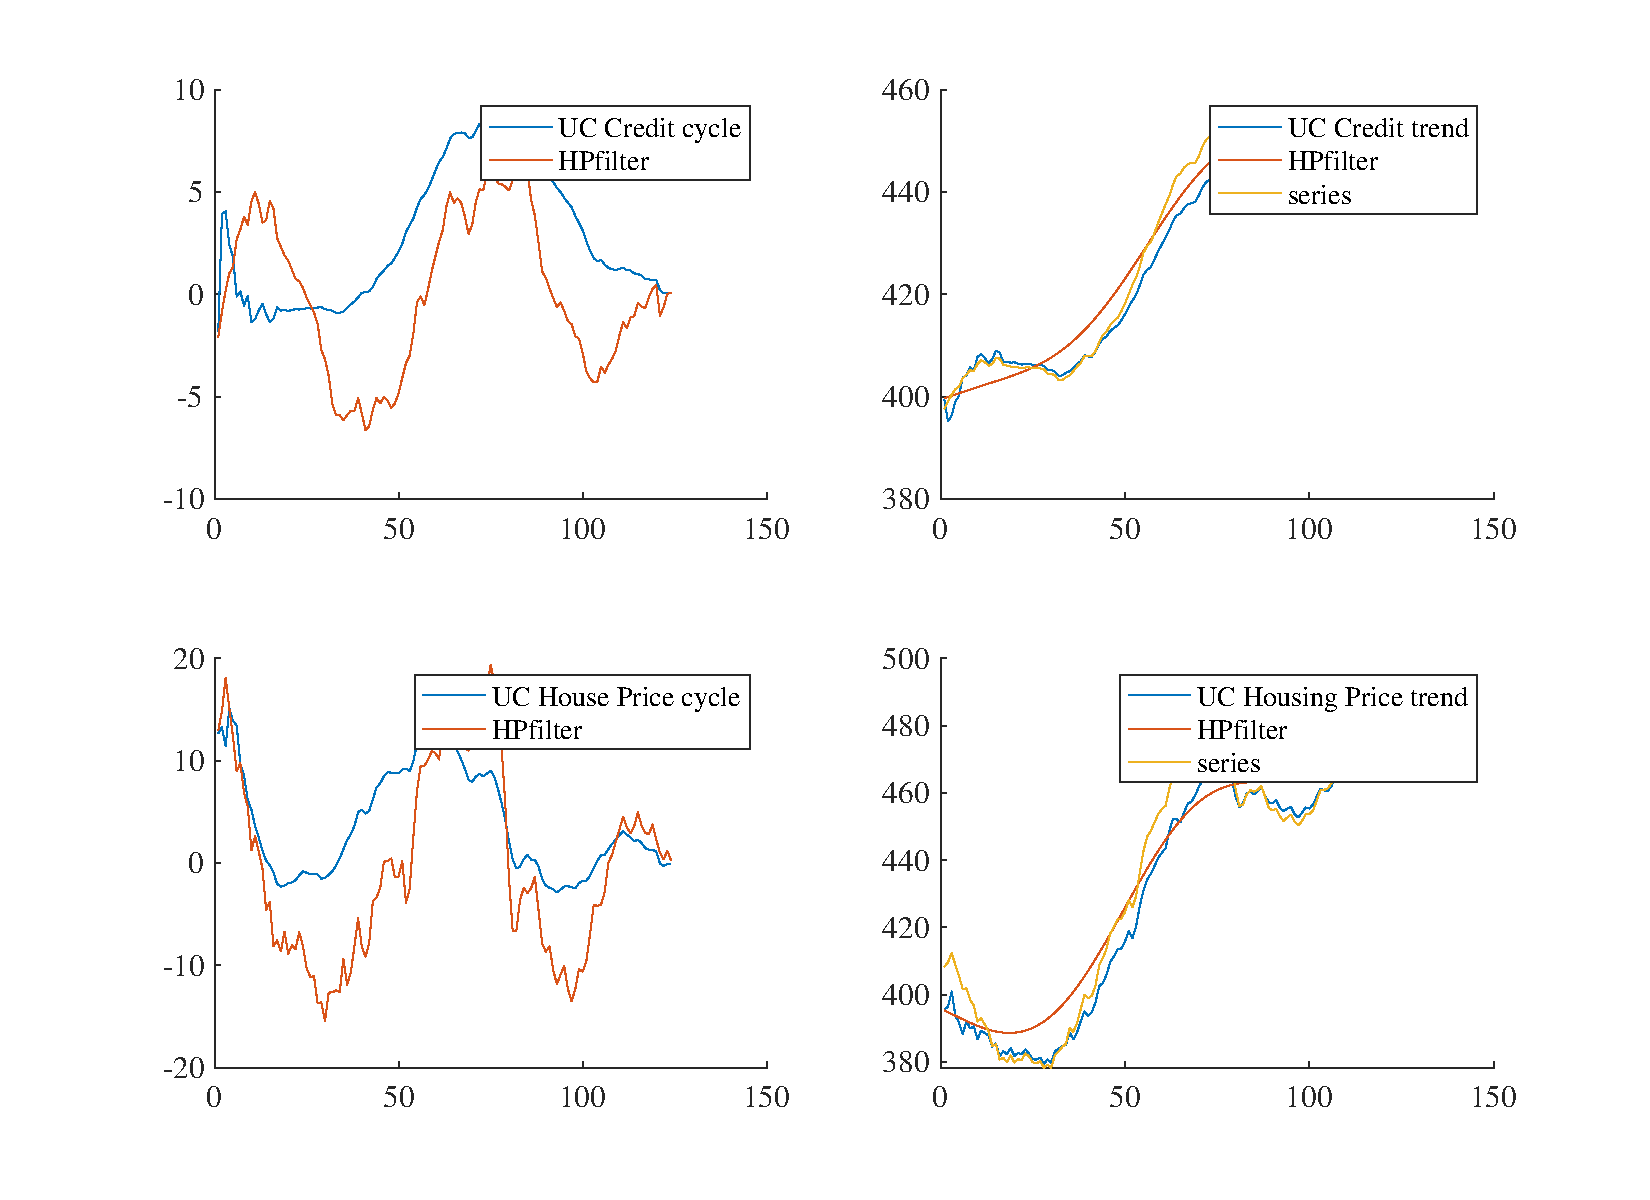
\includegraphics[width=0.85\linewidth]{../../Regression/Bayesian_UC_VAR2_nodrift/OutputData/cycles_GB} 

}

\caption{UK VAR(2)}\label{fig:unnamed-chunk-3}
\end{figure}

\begin{figure}

{\centering 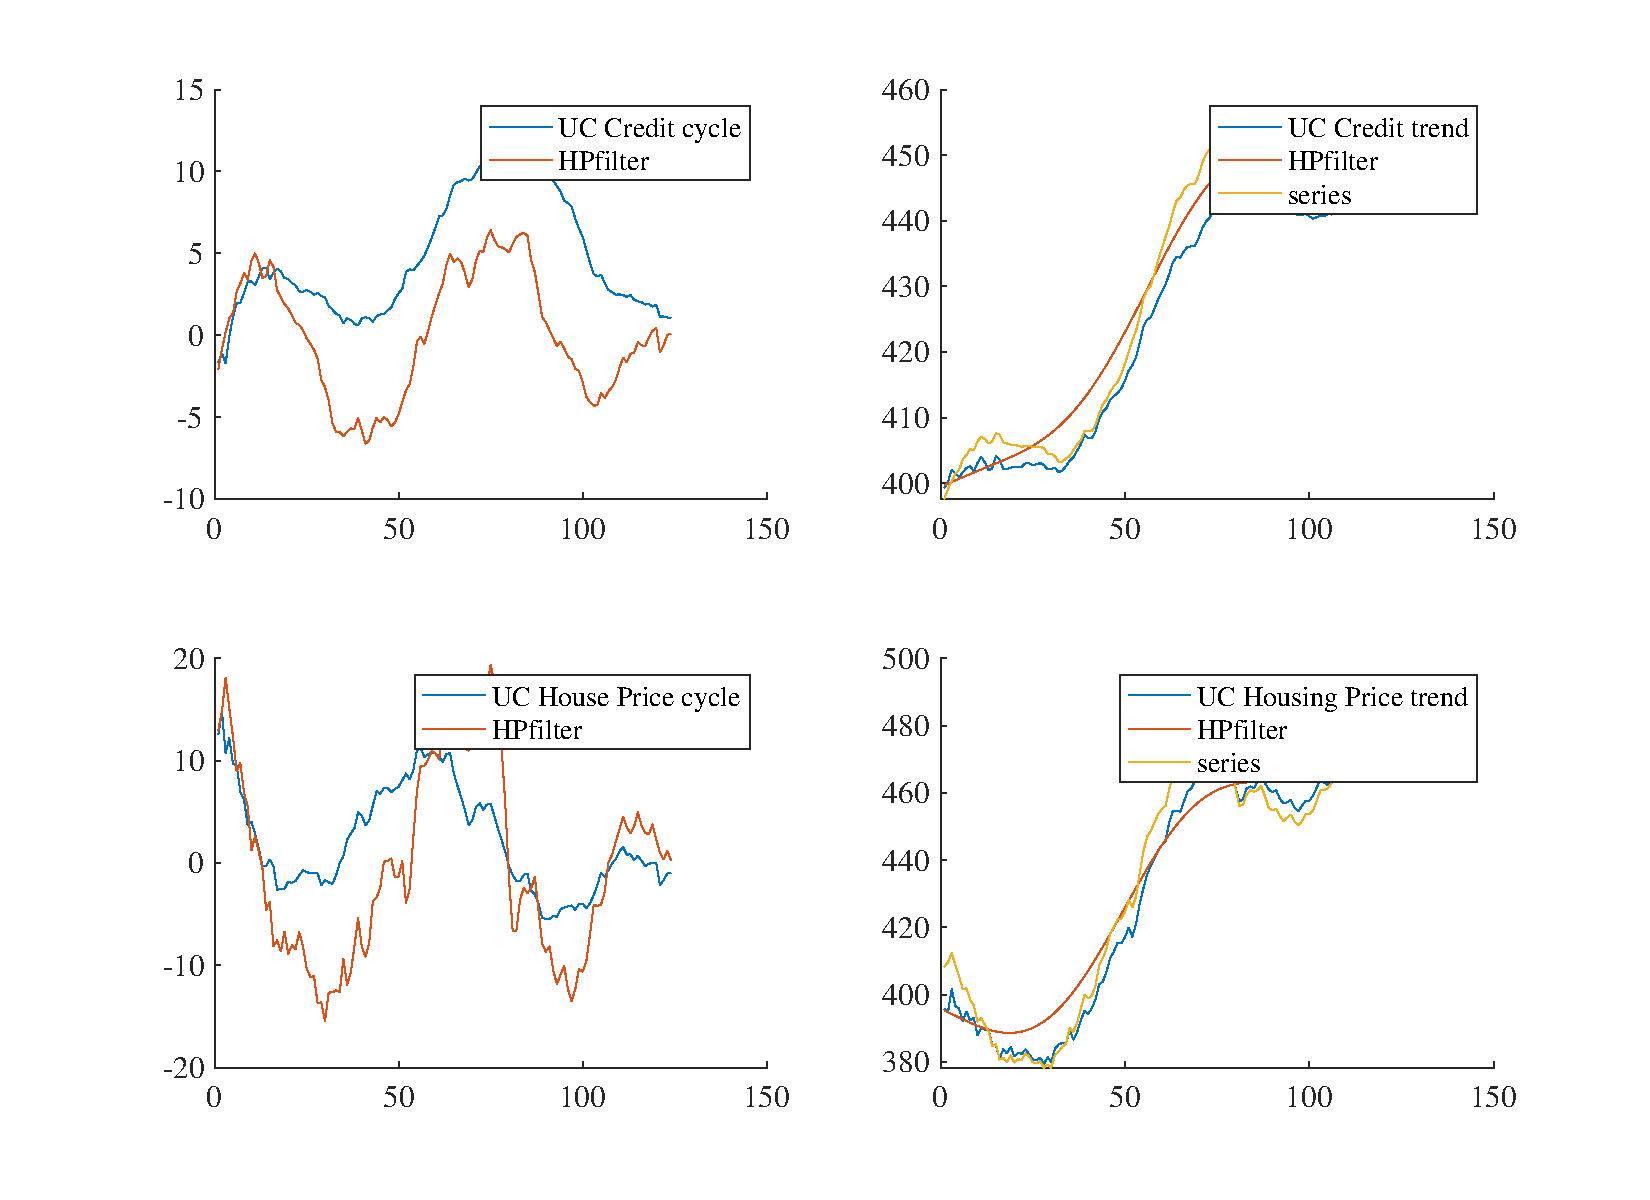
\includegraphics[width=0.85\linewidth]{../../Regression/Bayesian_UC_VAR2_nodrift_Crosscycle1lag/OutputData/cycles_GB} 

}

\caption{UK VAR(2) 1 cross-lag}\label{fig:unnamed-chunk-4}
\end{figure}

\begin{figure}

{\centering 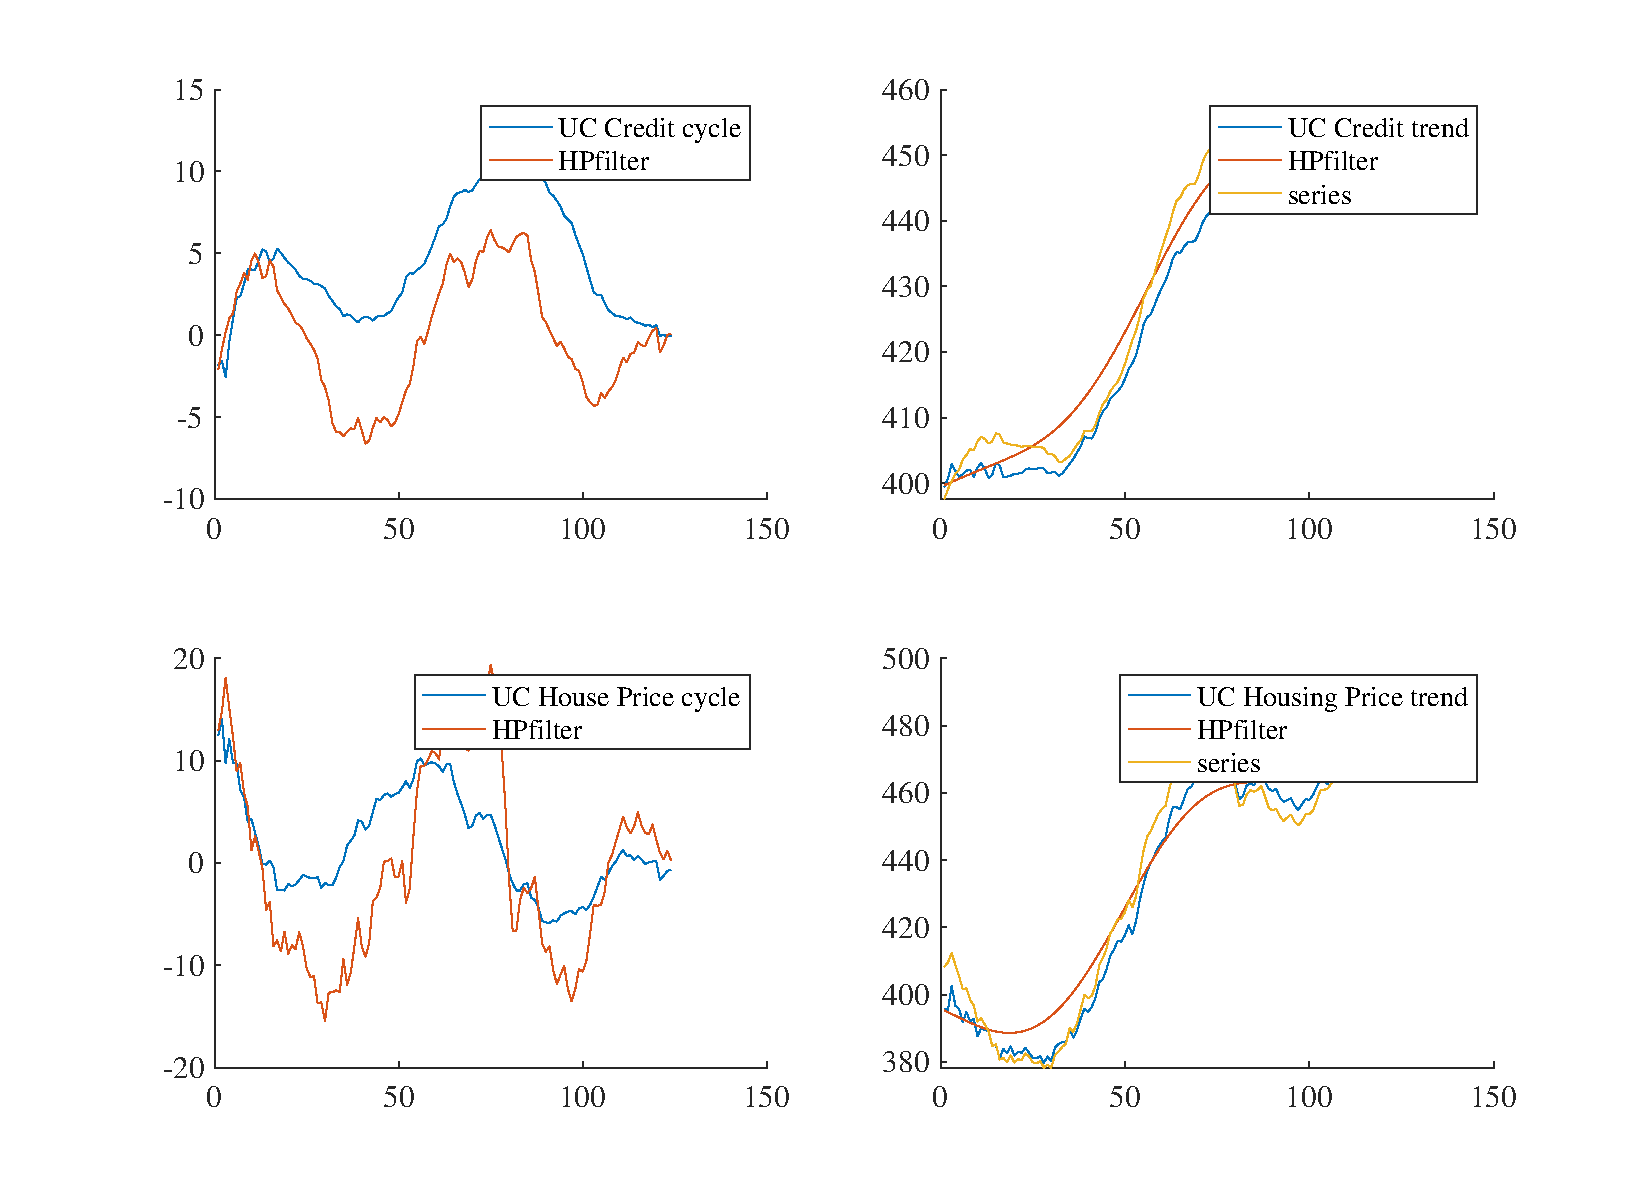
\includegraphics[width=0.85\linewidth]{../../Regression/Bayesian_UC_VAR2_nodrift_Crosscycle2lags/OutputData/cycles_GB} 

}

\caption{UK VAR(2) 2 cross-lags}\label{fig:unnamed-chunk-5}
\end{figure}

\clearpage

\hypertarget{us-graphs}{%
\subsection{US graphs}\label{us-graphs}}

\begin{figure}

{\centering 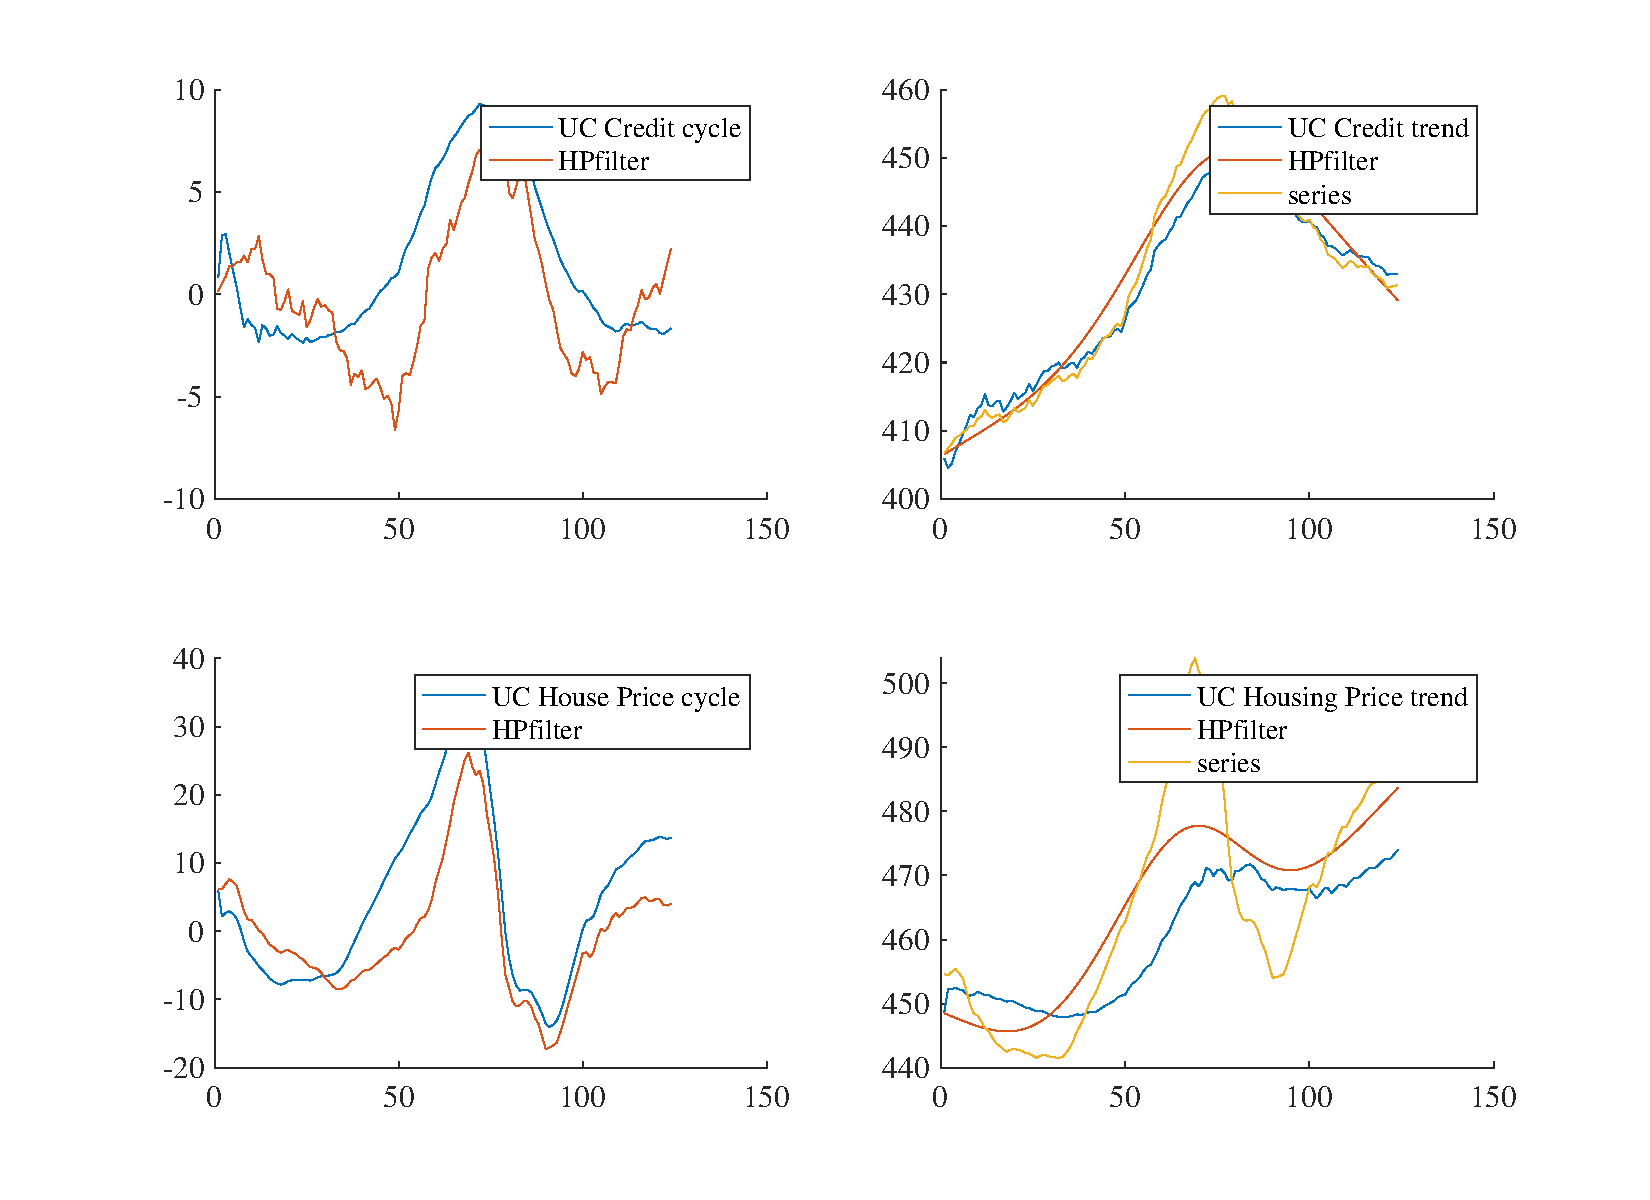
\includegraphics[width=0.85\linewidth]{../../Regression/Bayesian_UC_VAR2_nodrift/OutputData/cycles_US} 

}

\caption{US VAR(2)}\label{fig:unnamed-chunk-6}
\end{figure}

\begin{figure}

{\centering 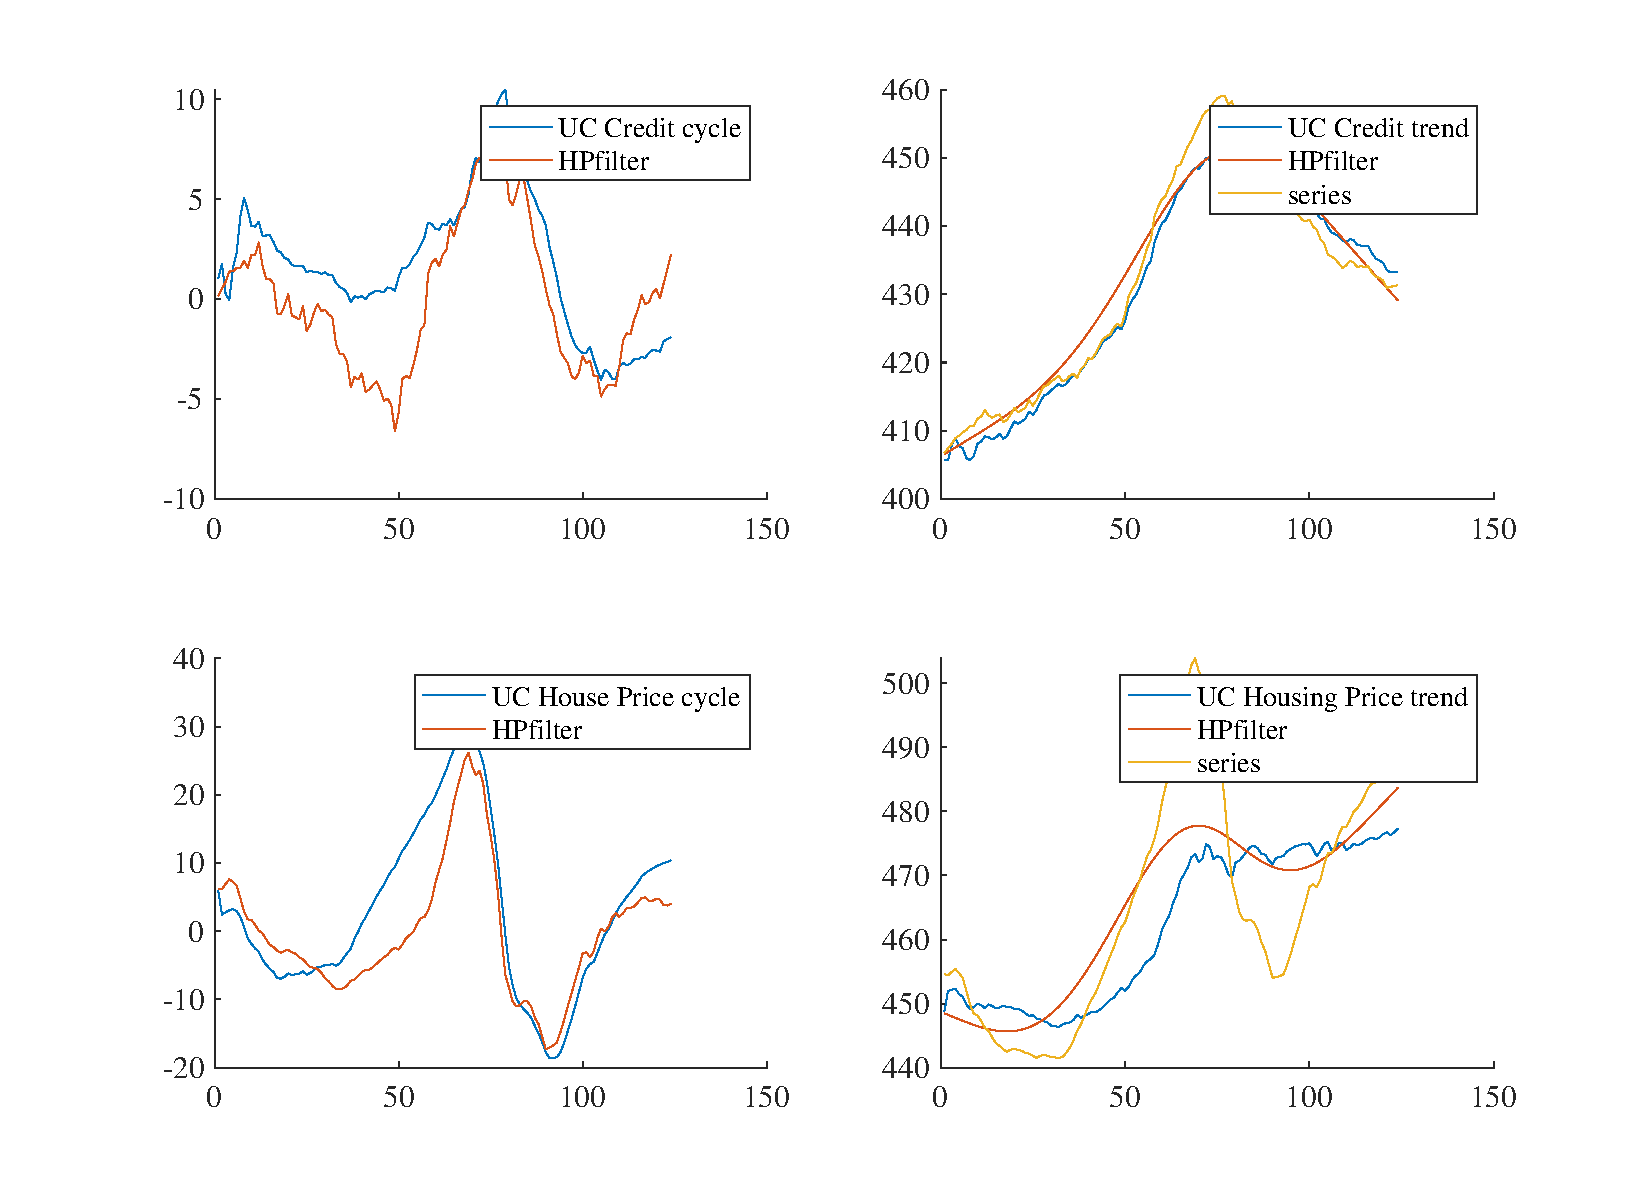
\includegraphics[width=0.85\linewidth]{../../Regression/Bayesian_UC_VAR2_nodrift_Crosscycle1lag/OutputData/cycles_US} 

}

\caption{US VAR(2) 1 cross-lag}\label{fig:unnamed-chunk-7}
\end{figure}

\begin{figure}

{\centering 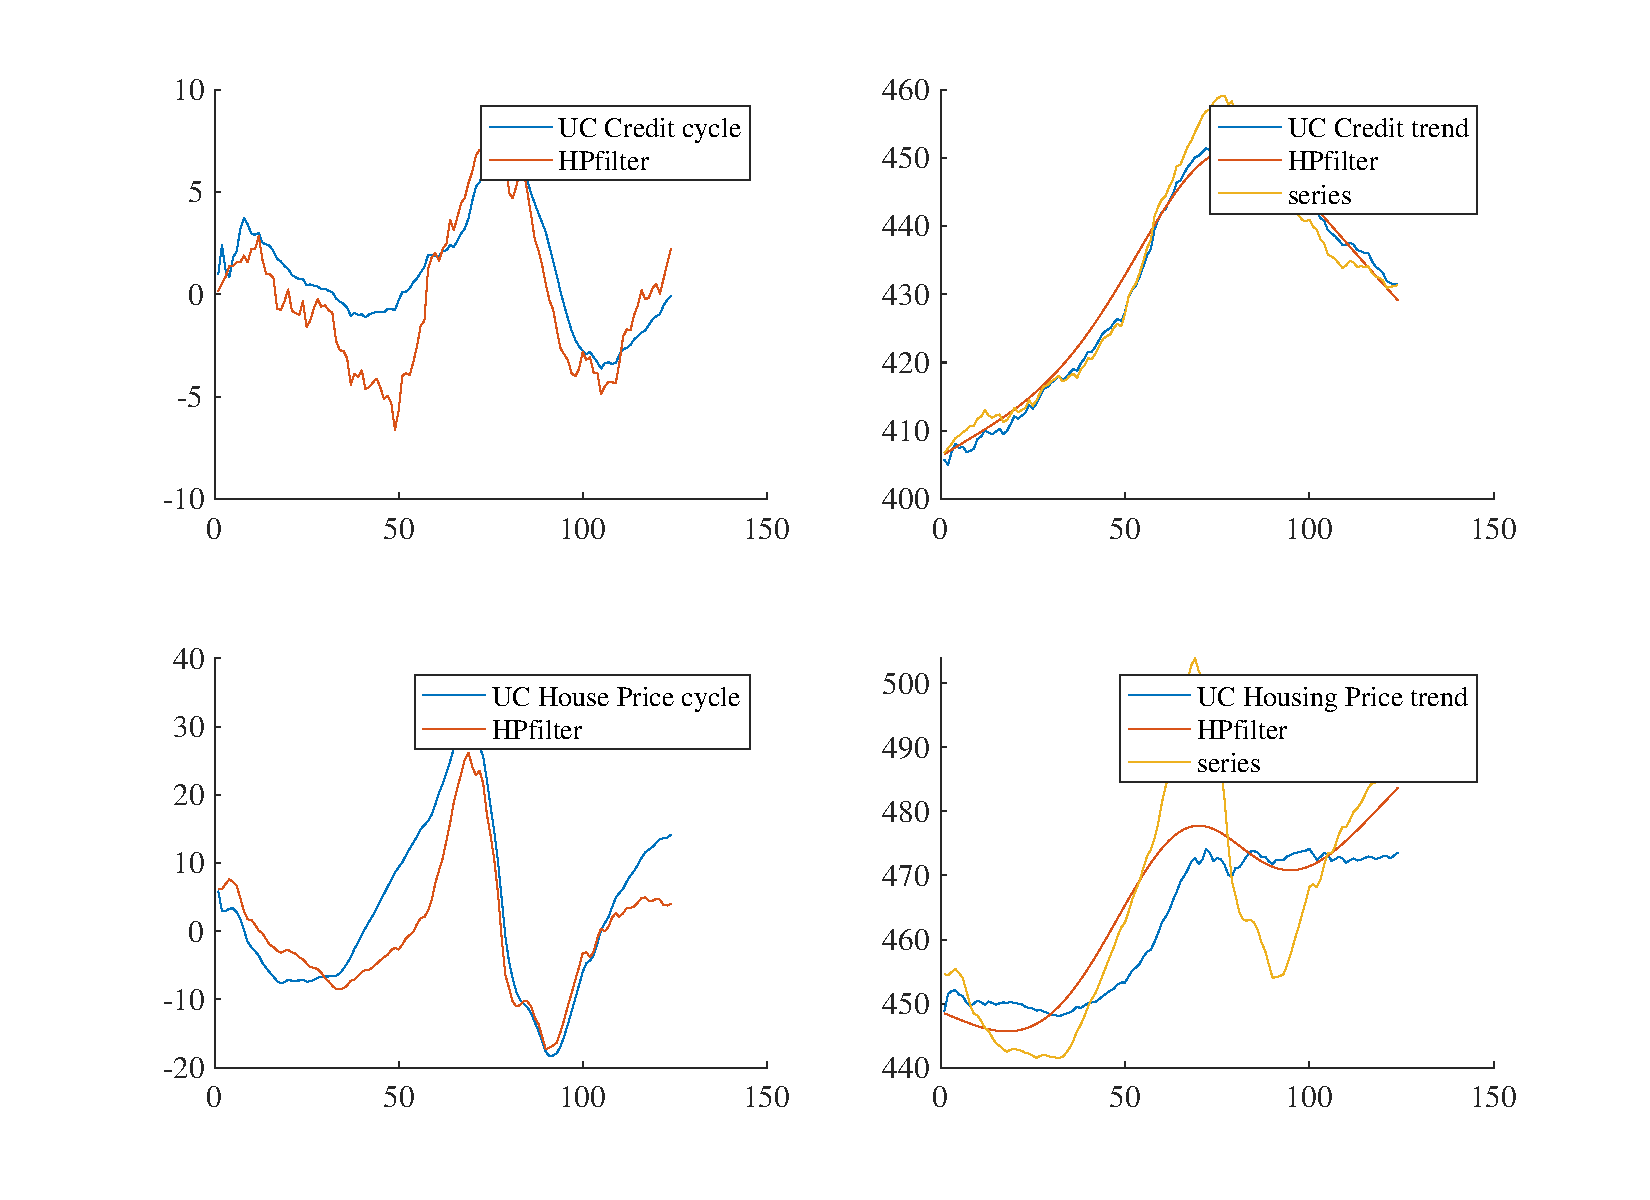
\includegraphics[width=0.85\linewidth]{../../Regression/Bayesian_UC_VAR2_nodrift_Crosscycle2lags/OutputData/cycles_US} 

}

\caption{US VAR(2) 2 cross-lags}\label{fig:unnamed-chunk-8}
\end{figure}

\clearpage

\hypertarget{posterior-and-prior-distribution}{%
\section{Posterior and Prior Distribution}\label{posterior-and-prior-distribution}}

\hypertarget{uk-posterior-and-prior-distribution}{%
\subsection{UK Posterior and Prior Distribution}\label{uk-posterior-and-prior-distribution}}

\begin{figure}

{\centering 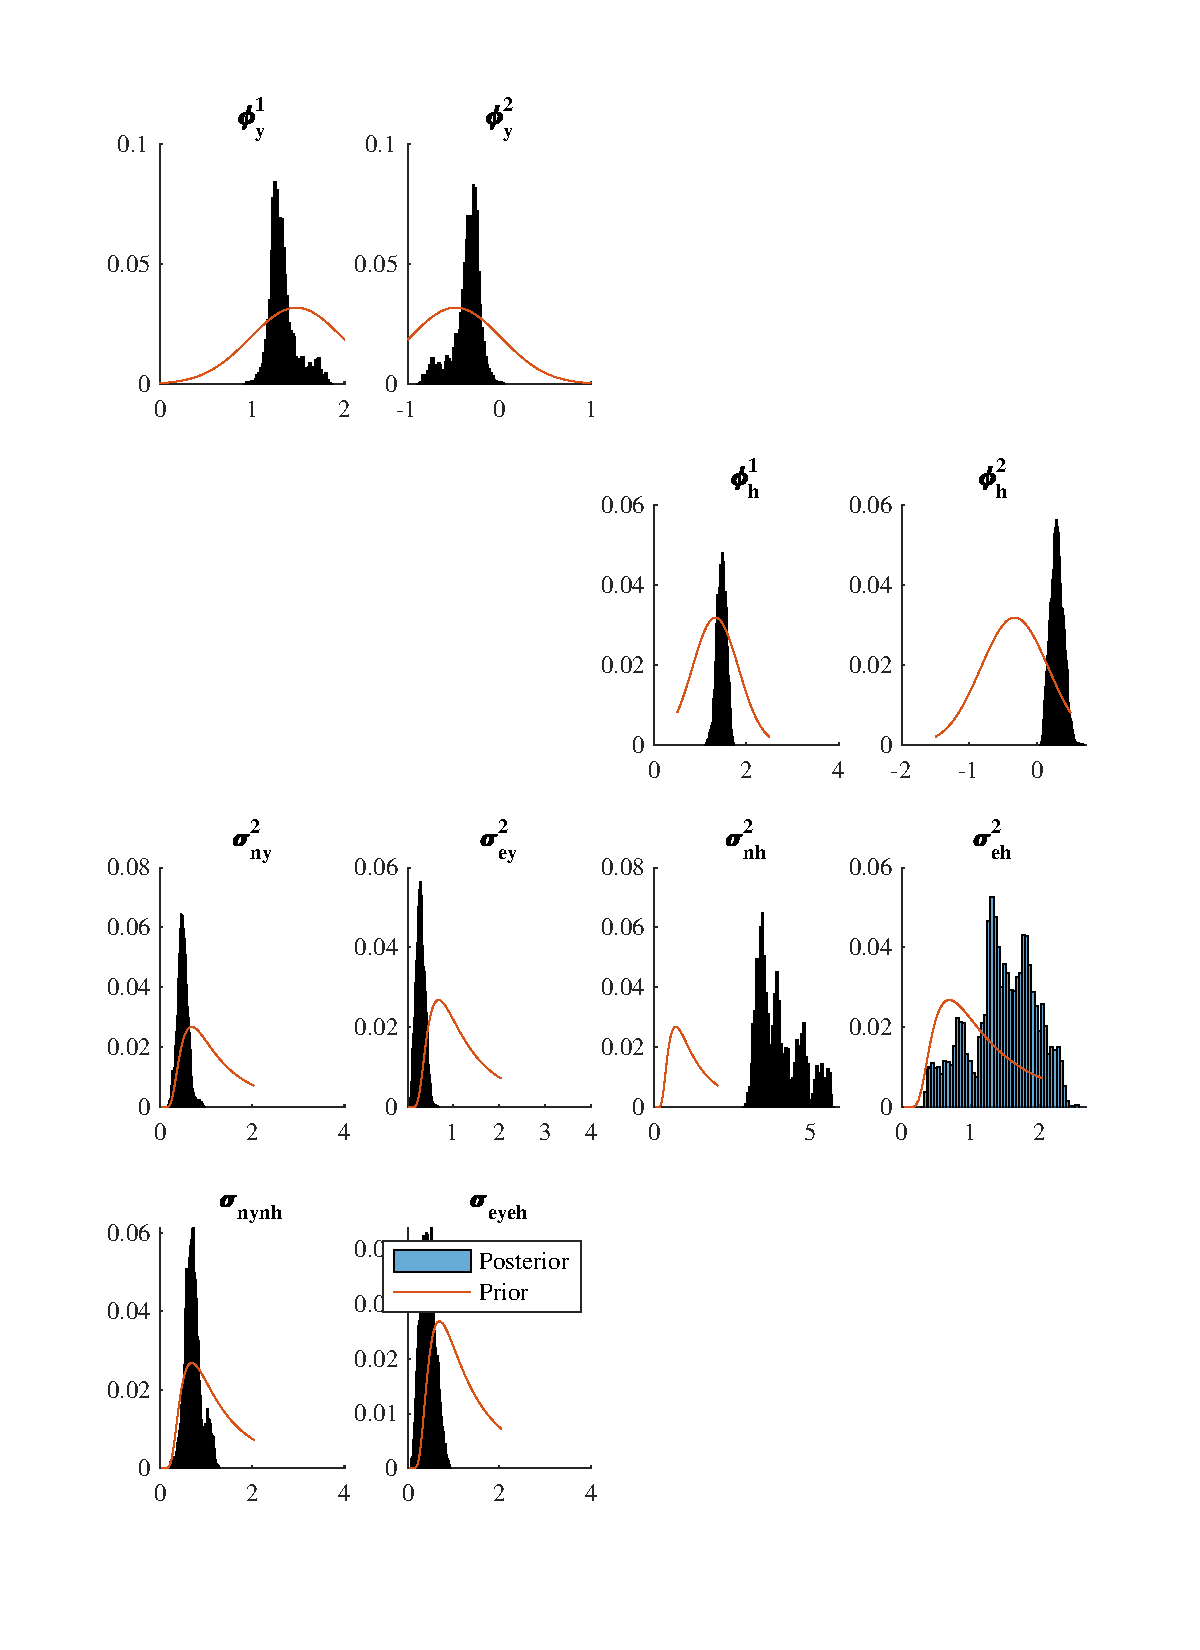
\includegraphics[width=0.85\linewidth]{../../Regression/Bayesian_UC_VAR2_nodrift/OutputData/posteriorpriordistribution_GB} 

}

\caption{UK VAR(2)}\label{fig:unnamed-chunk-9}
\end{figure}

\begin{figure}

{\centering 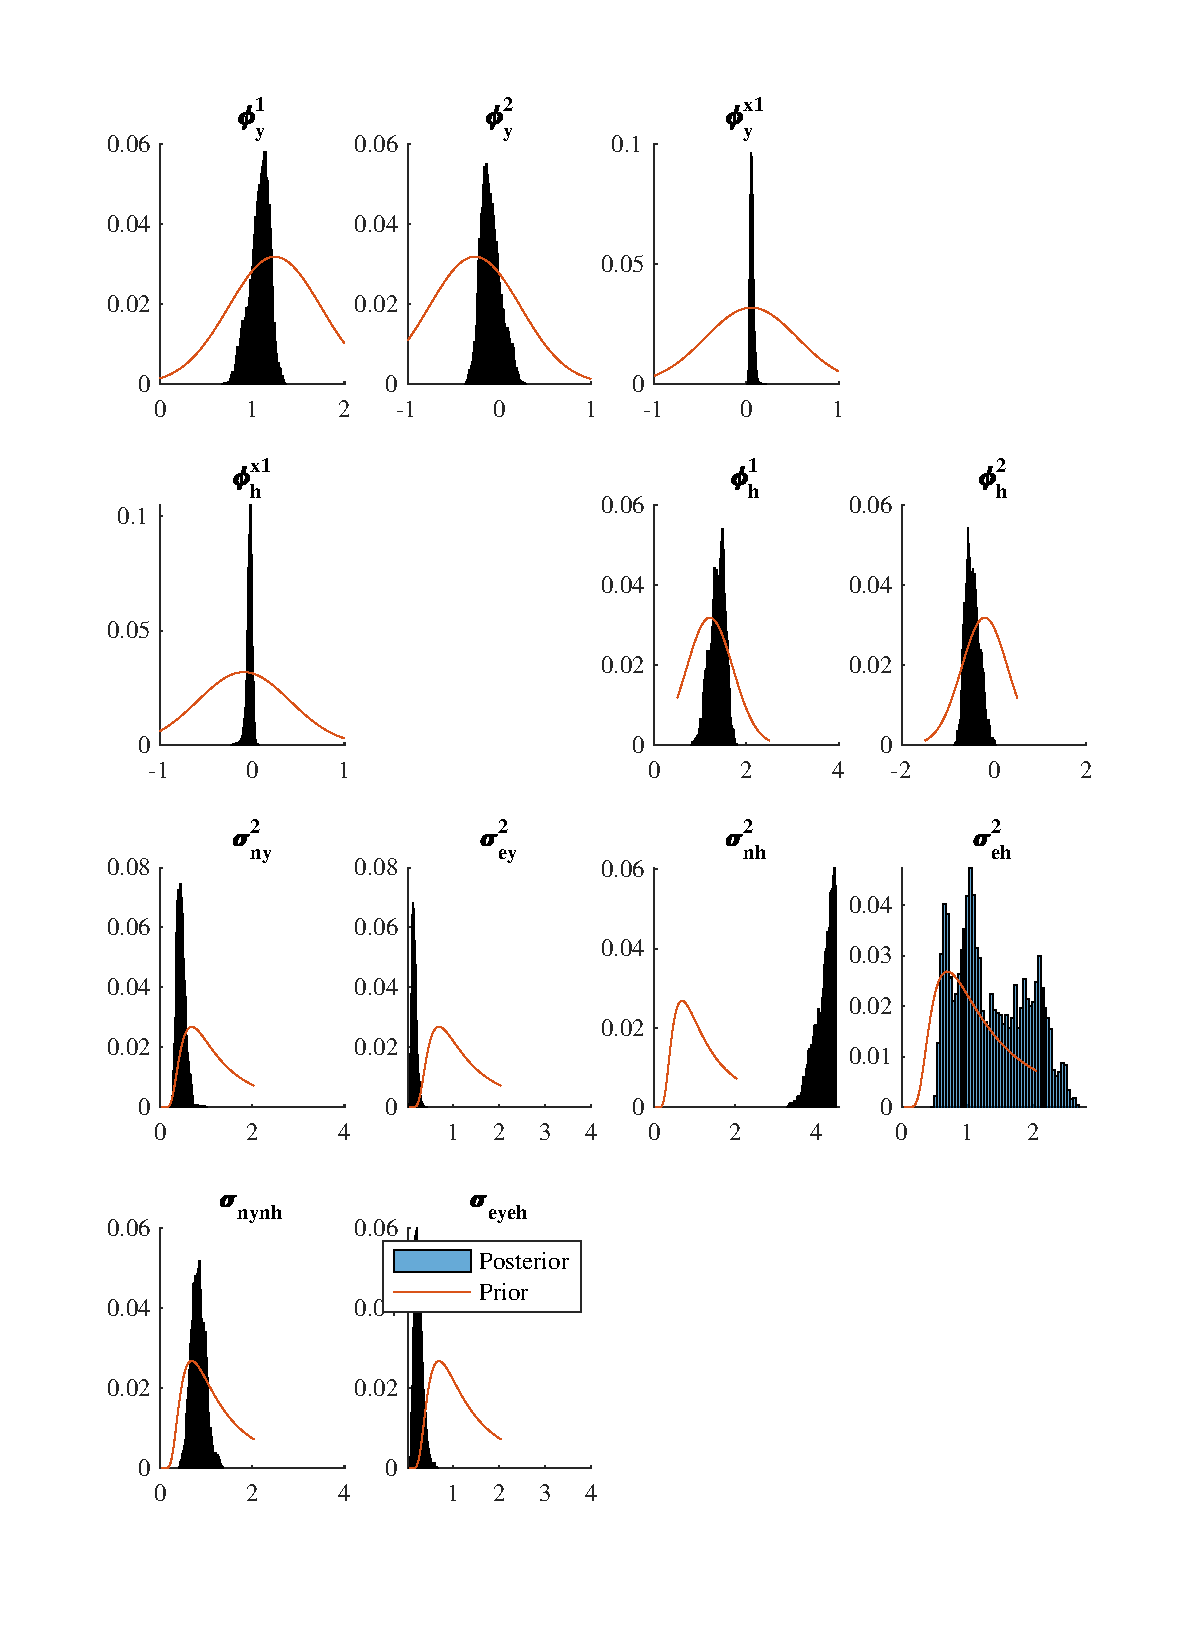
\includegraphics[width=0.85\linewidth]{../../Regression/Bayesian_UC_VAR2_nodrift_Crosscycle1lag/OutputData/posteriorpriordistribution_GB} 

}

\caption{UK VAR(2) 1 cross-lag}\label{fig:unnamed-chunk-10}
\end{figure}

\begin{figure}

{\centering 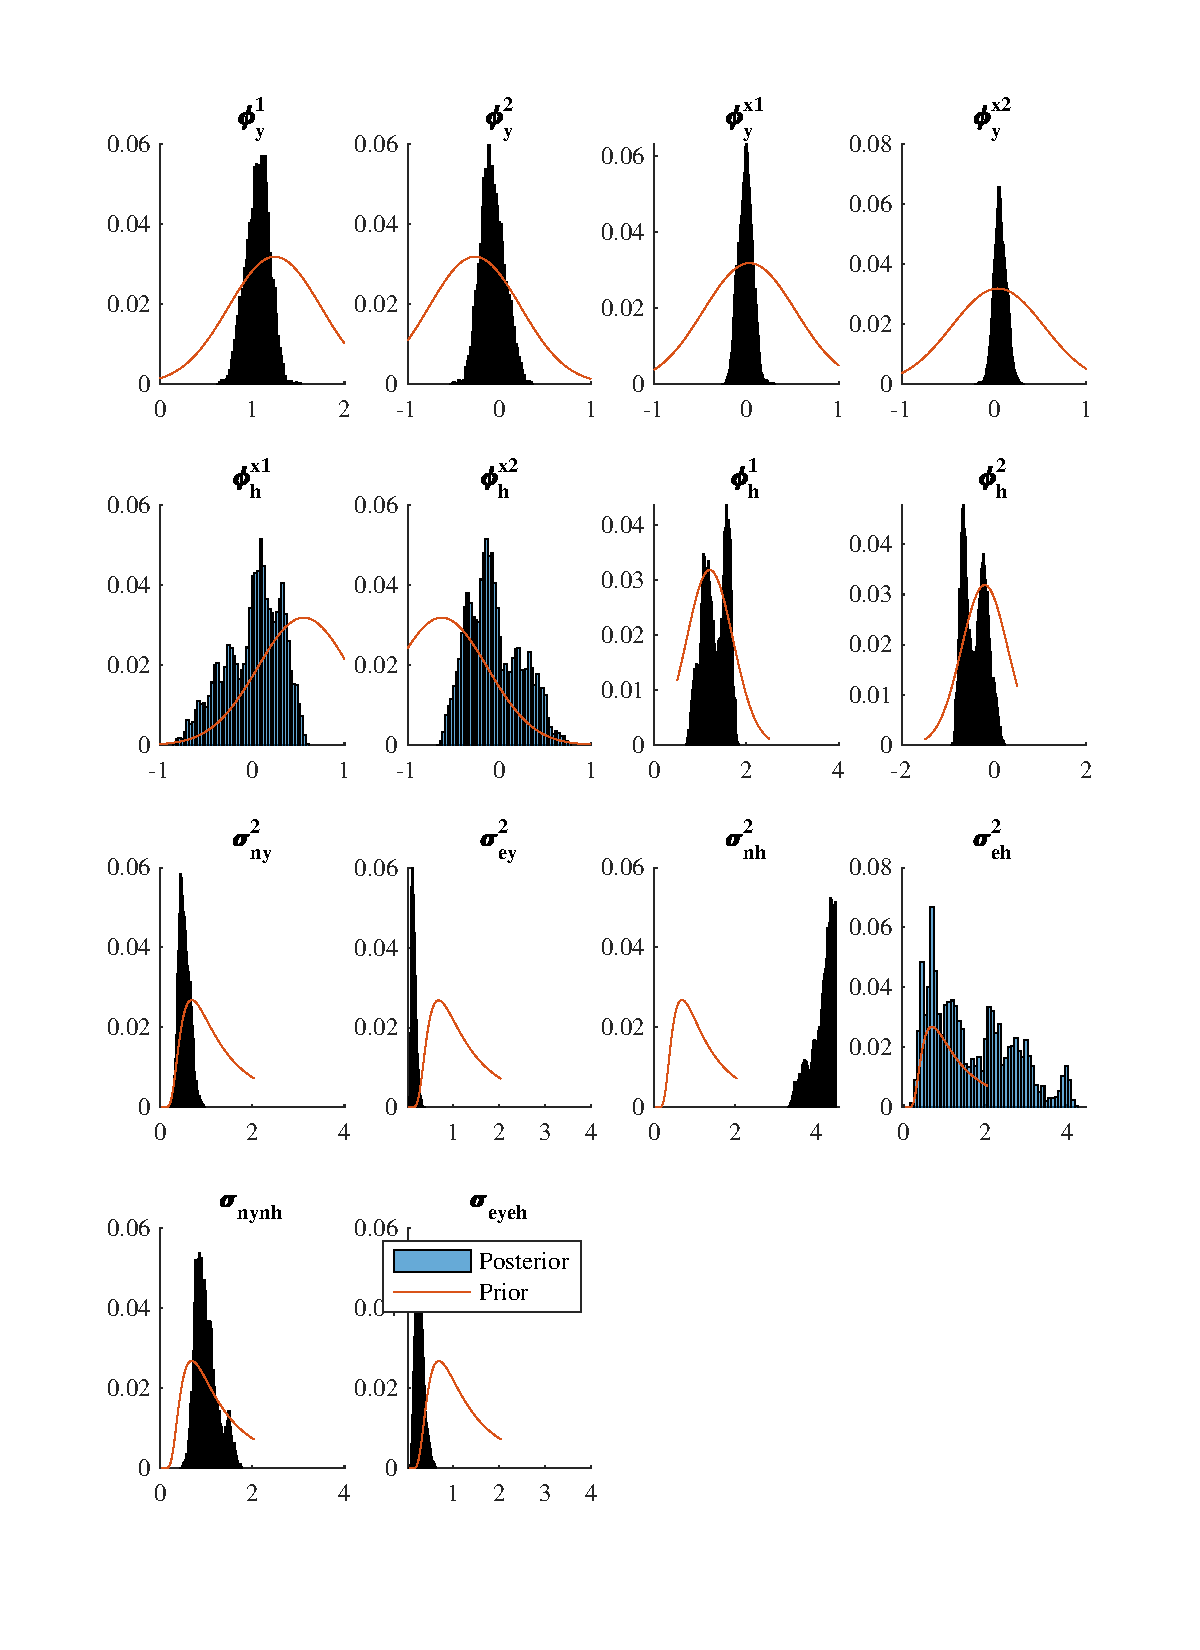
\includegraphics[width=0.85\linewidth]{../../Regression/Bayesian_UC_VAR2_nodrift_Crosscycle2lags/OutputData/posteriorpriordistribution_GB} 

}

\caption{UK VAR(2) 2 cross-lags}\label{fig:unnamed-chunk-11}
\end{figure}

\clearpage

\hypertarget{us-posterior-and-prior-distribution}{%
\subsection{US Posterior and Prior Distribution}\label{us-posterior-and-prior-distribution}}

\begin{figure}

{\centering 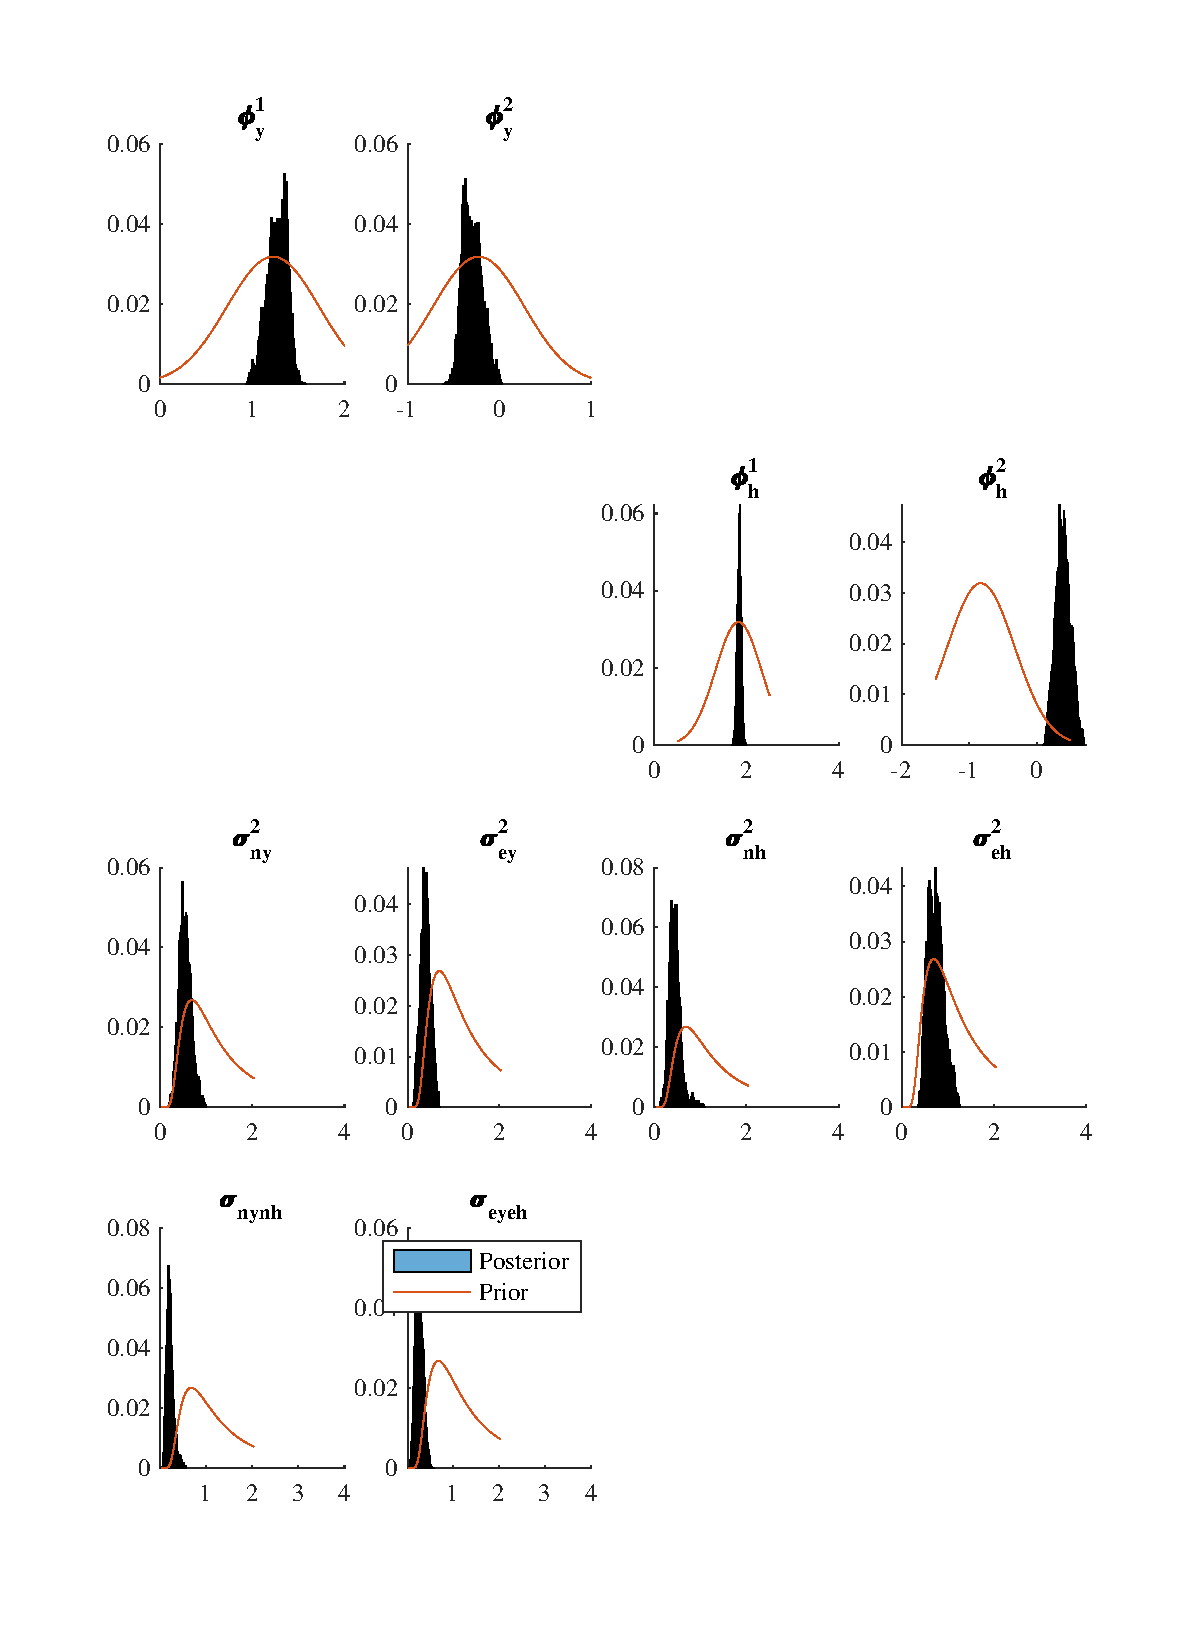
\includegraphics[width=0.85\linewidth]{../../Regression/Bayesian_UC_VAR2_nodrift/OutputData/posteriorpriordistribution_US} 

}

\caption{US VAR(2)}\label{fig:unnamed-chunk-12}
\end{figure}

\begin{figure}

{\centering 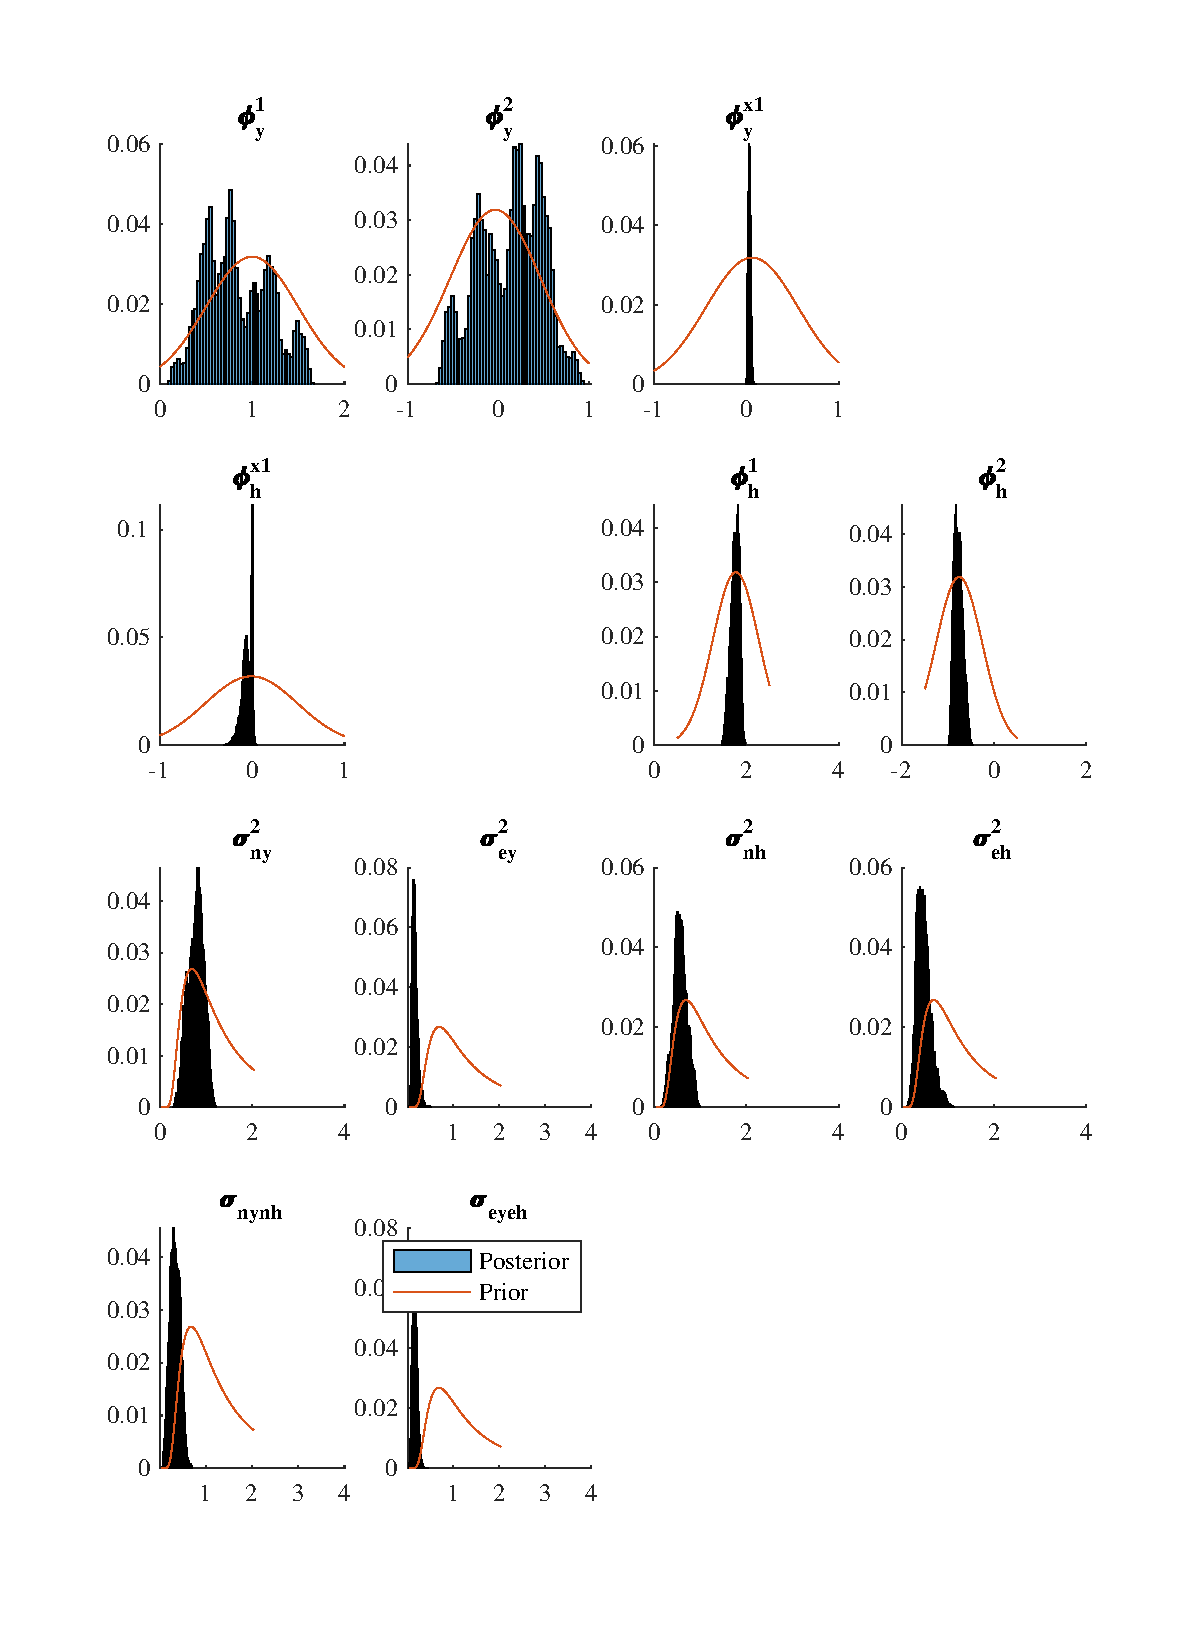
\includegraphics[width=0.85\linewidth]{../../Regression/Bayesian_UC_VAR2_nodrift_Crosscycle1lag/OutputData/posteriorpriordistribution_US} 

}

\caption{US VAR(2) 1 cross-lag}\label{fig:unnamed-chunk-13}
\end{figure}

\begin{figure}

{\centering 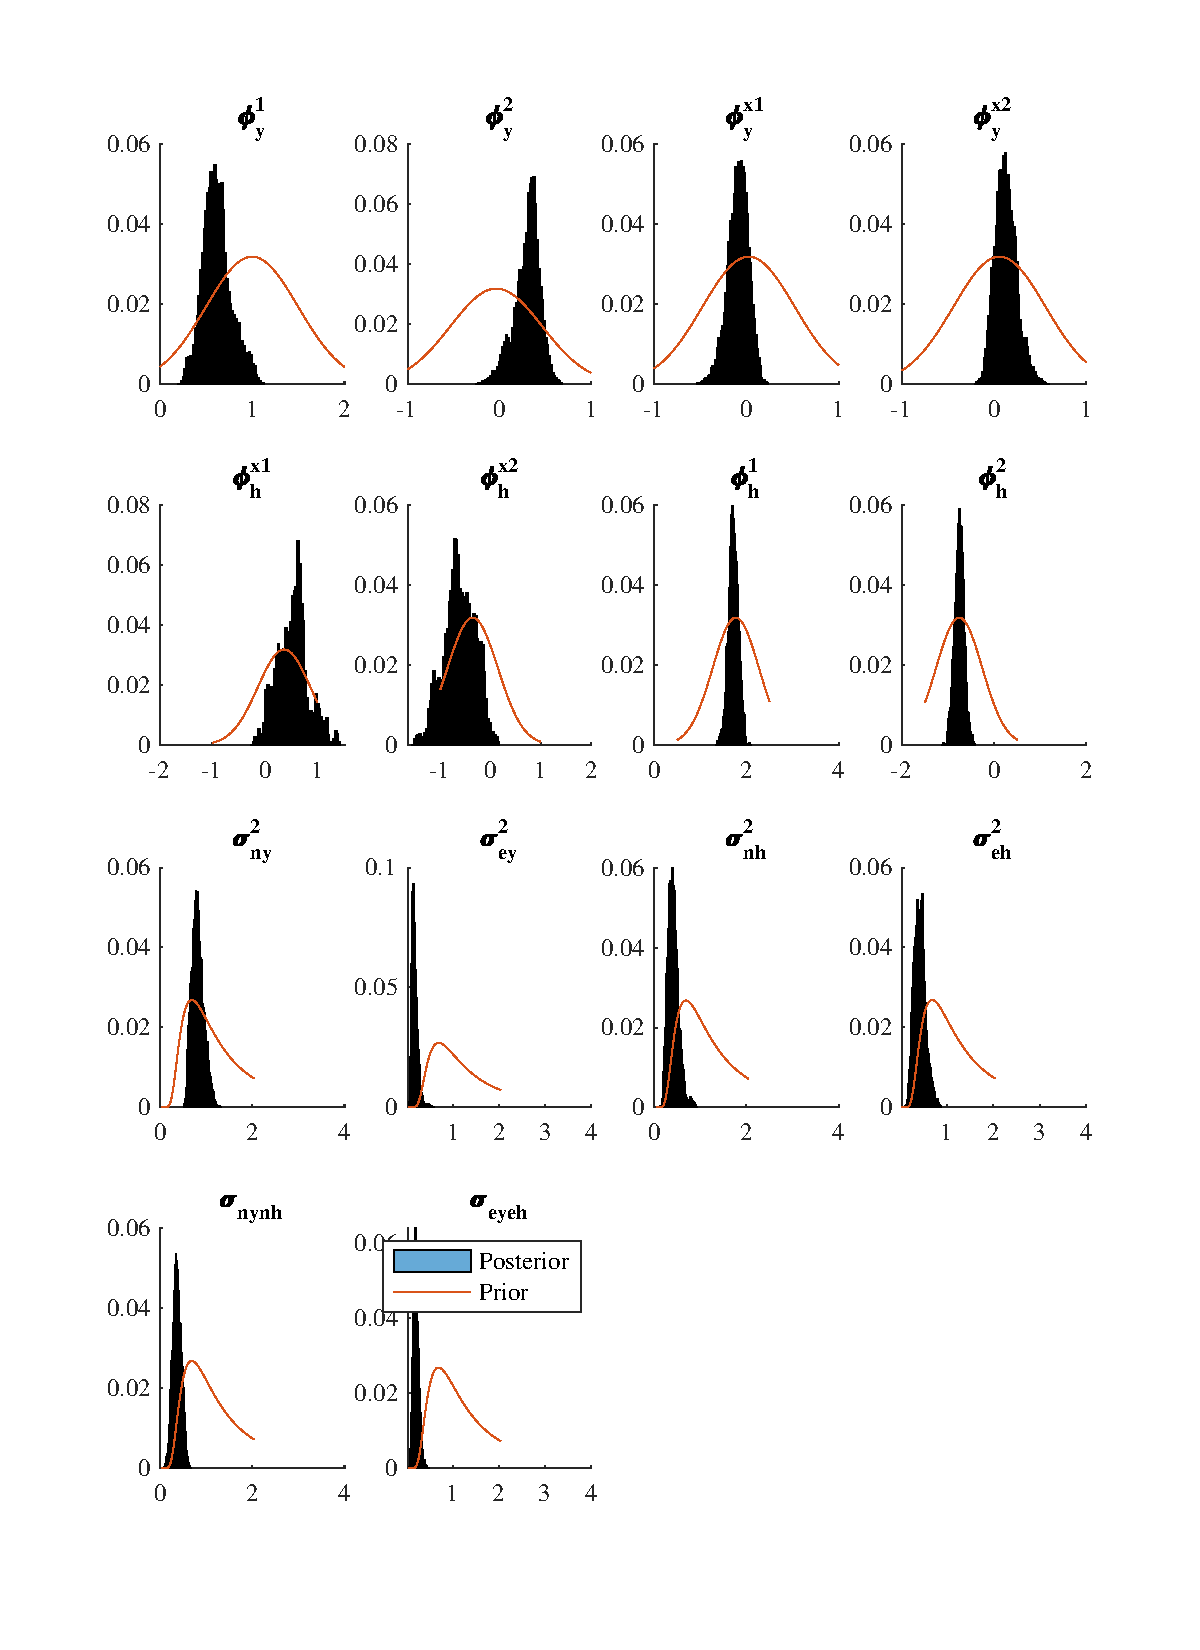
\includegraphics[width=0.85\linewidth]{../../Regression/Bayesian_UC_VAR2_nodrift_Crosscycle2lags/OutputData/posteriorpriordistribution_US} 

}

\caption{US VAR(2) 2 cross-lags}\label{fig:unnamed-chunk-14}
\end{figure}

\clearpage

\hypertarget{posterior-chain}{%
\section{Posterior chain}\label{posterior-chain}}

\hypertarget{uk-posterior-chain}{%
\subsection{UK Posterior chain}\label{uk-posterior-chain}}

\begin{figure}

{\centering 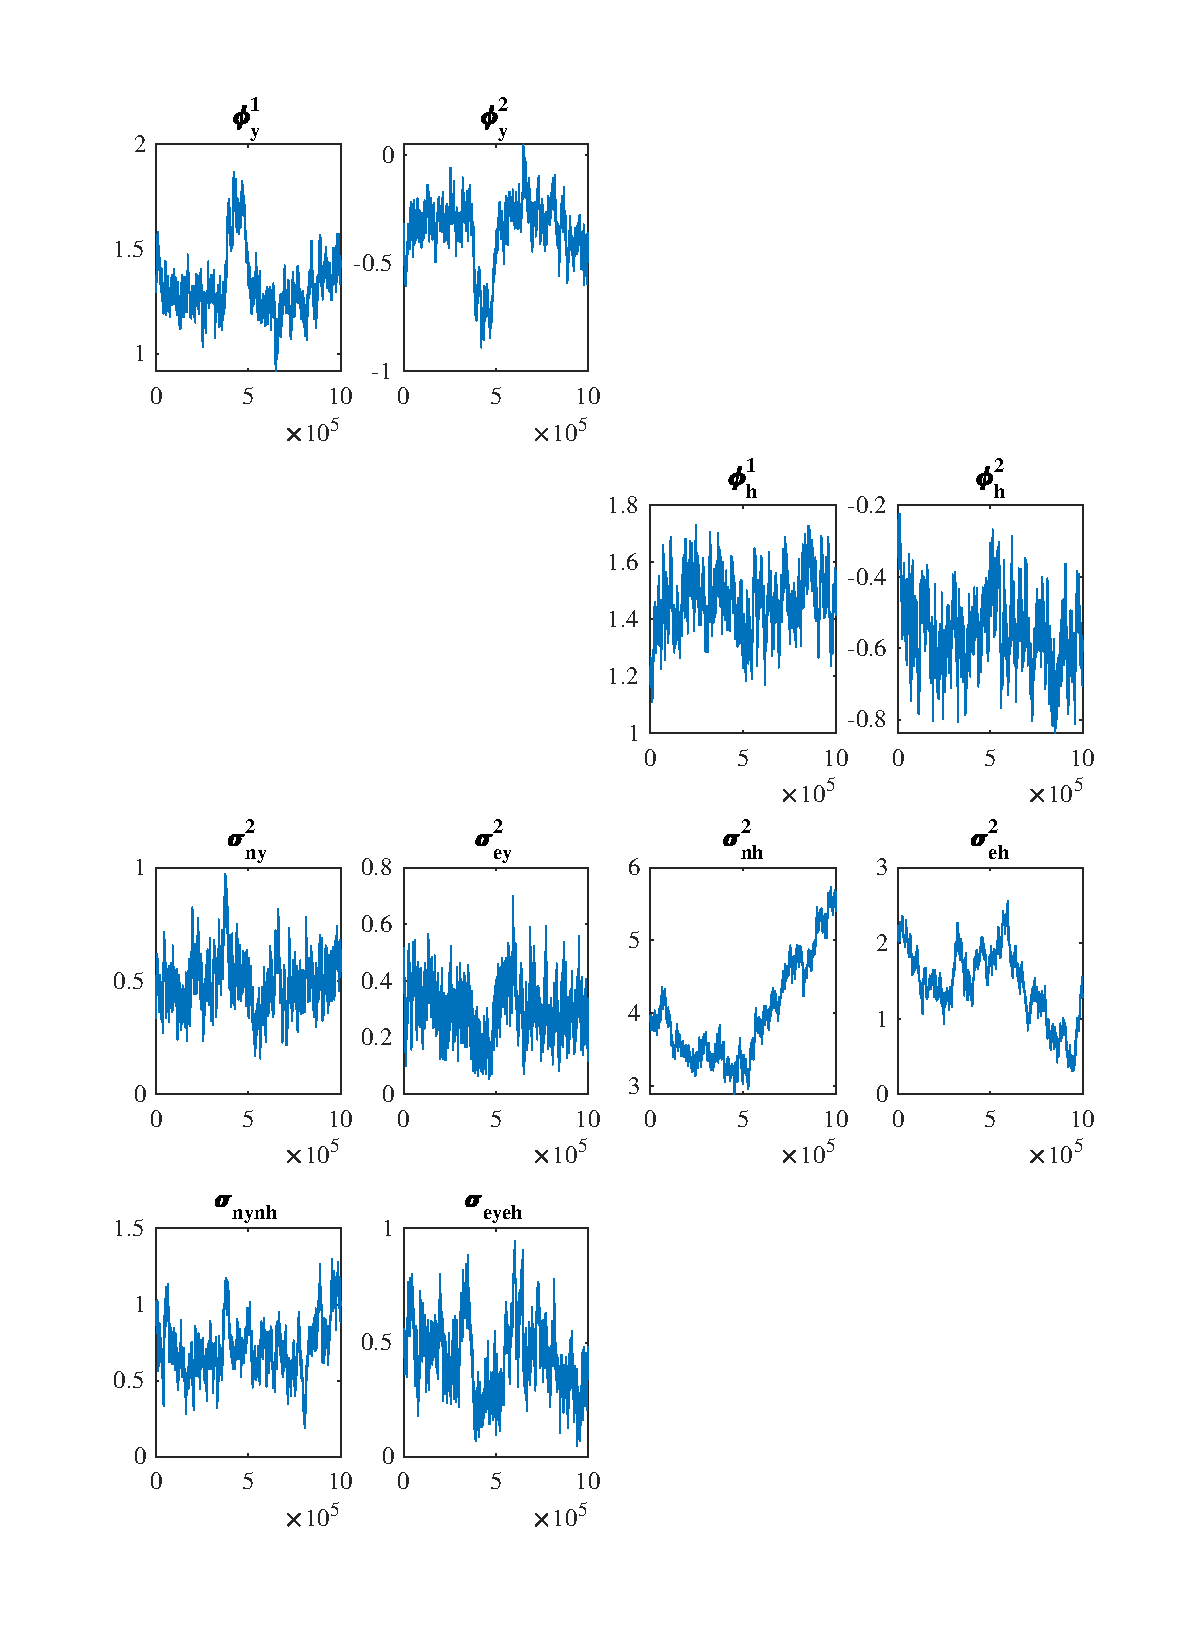
\includegraphics[width=0.85\linewidth]{../../Regression/Bayesian_UC_VAR2_nodrift/OutputData/posteriorchain_GB} 

}

\caption{UK VAR(2)}\label{fig:unnamed-chunk-15}
\end{figure}

\begin{figure}

{\centering 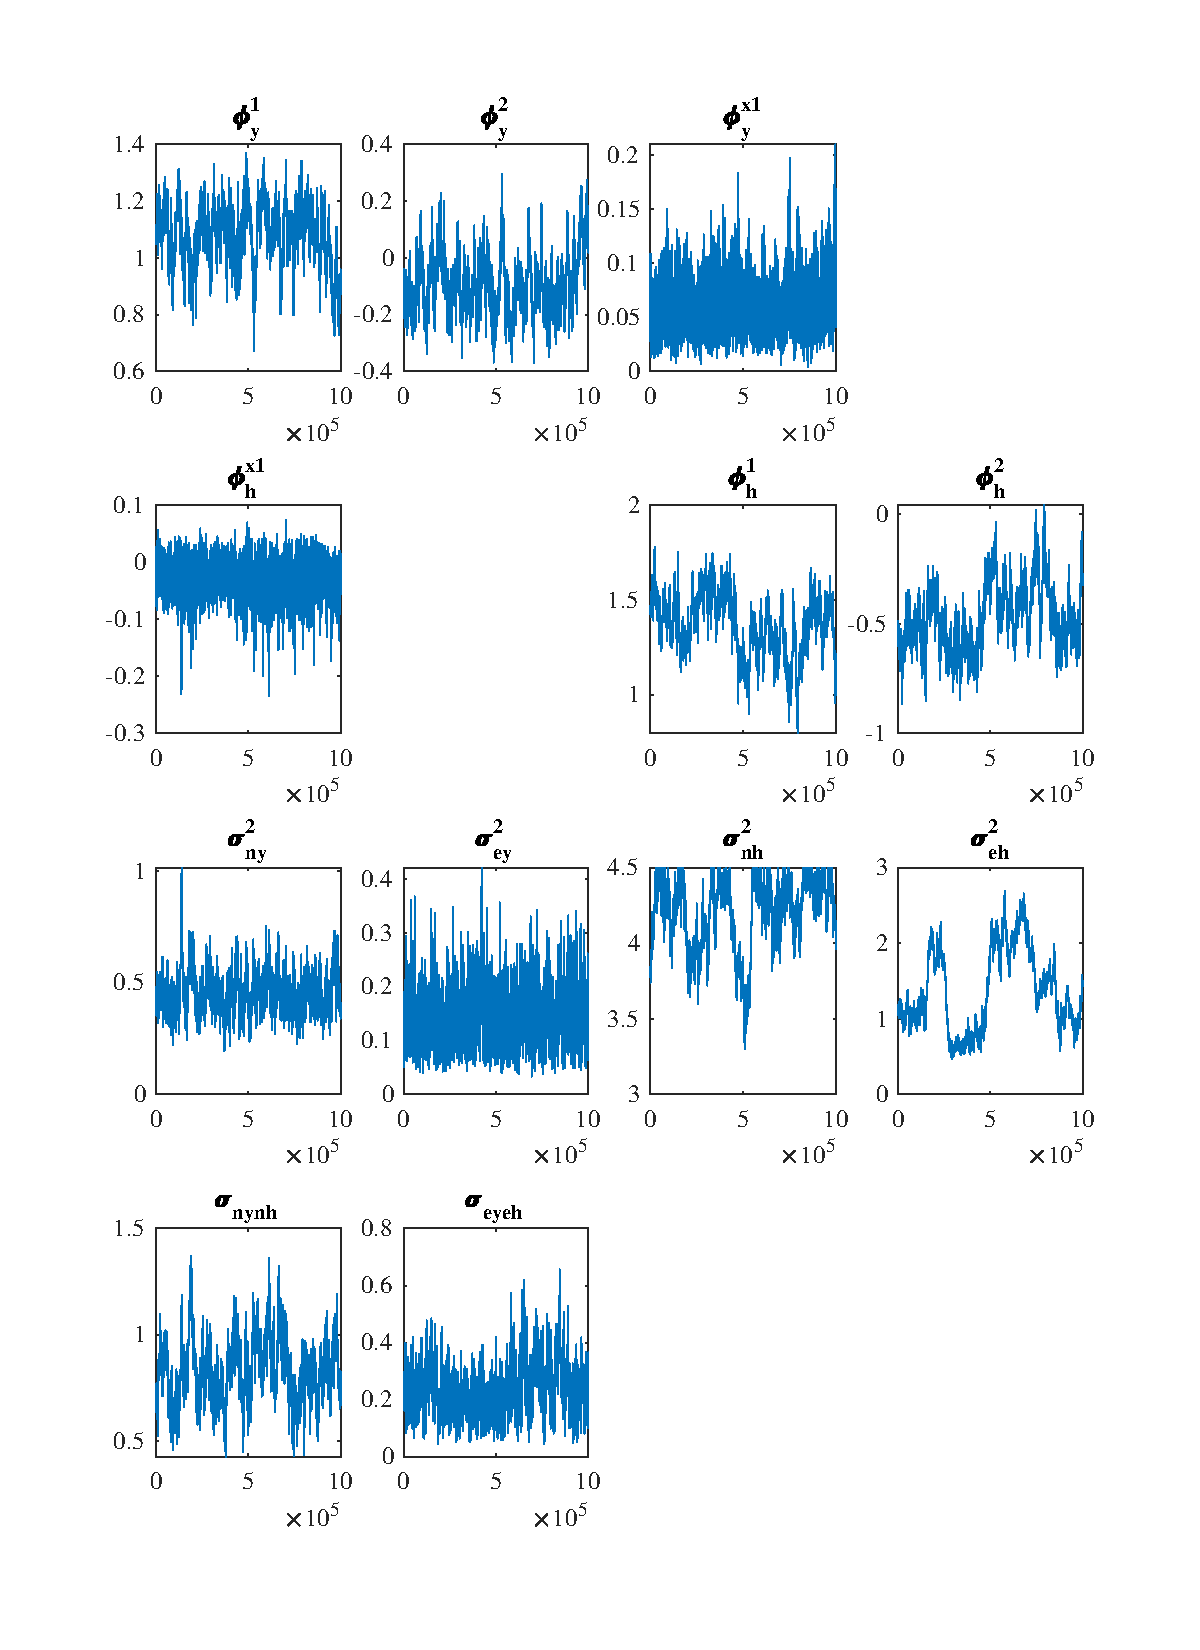
\includegraphics[width=0.85\linewidth]{../../Regression/Bayesian_UC_VAR2_nodrift_Crosscycle1lag/OutputData/posteriorchain_GB} 

}

\caption{UK VAR(2) 1 cross-lag}\label{fig:unnamed-chunk-16}
\end{figure}

\begin{figure}

{\centering 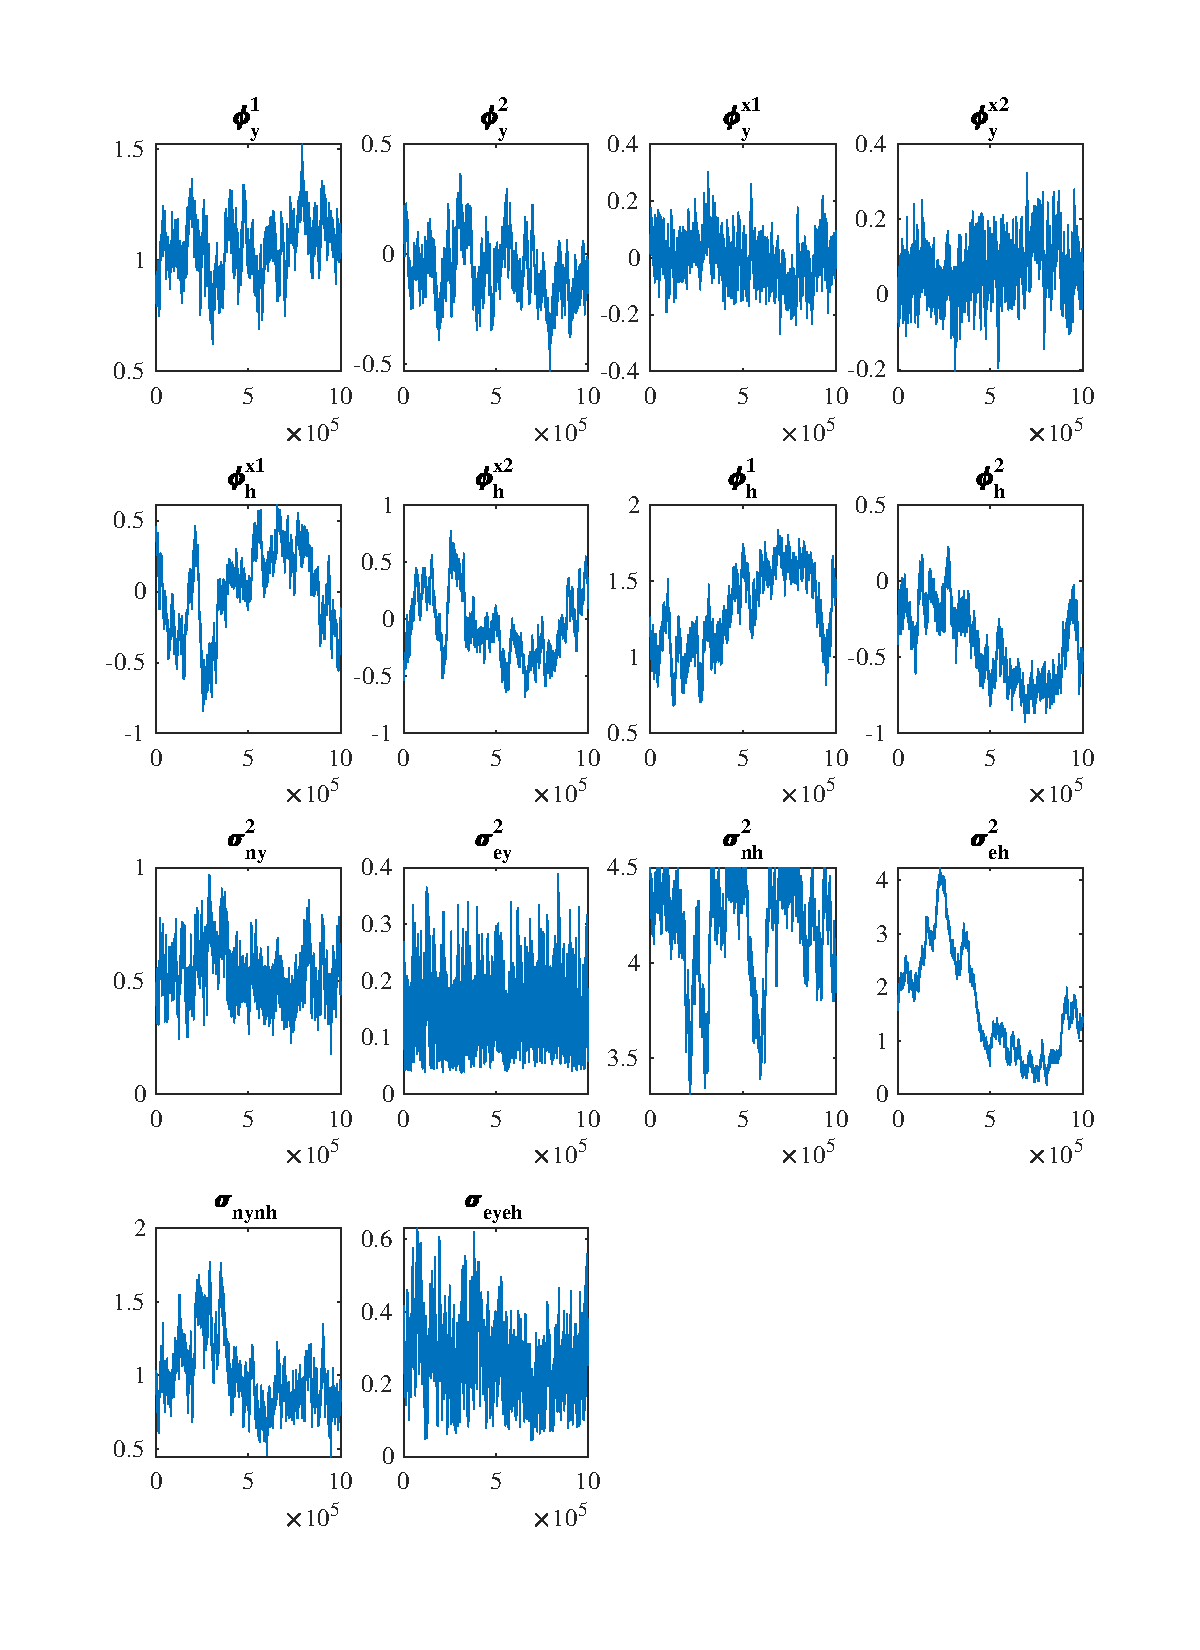
\includegraphics[width=0.85\linewidth]{../../Regression/Bayesian_UC_VAR2_nodrift_Crosscycle2lags/OutputData/posteriorchain_GB} 

}

\caption{UK VAR(2) 2 cross-lags}\label{fig:unnamed-chunk-17}
\end{figure}

\clearpage

\hypertarget{us-posterior-chain}{%
\subsection{US Posterior chain}\label{us-posterior-chain}}

\begin{figure}

{\centering 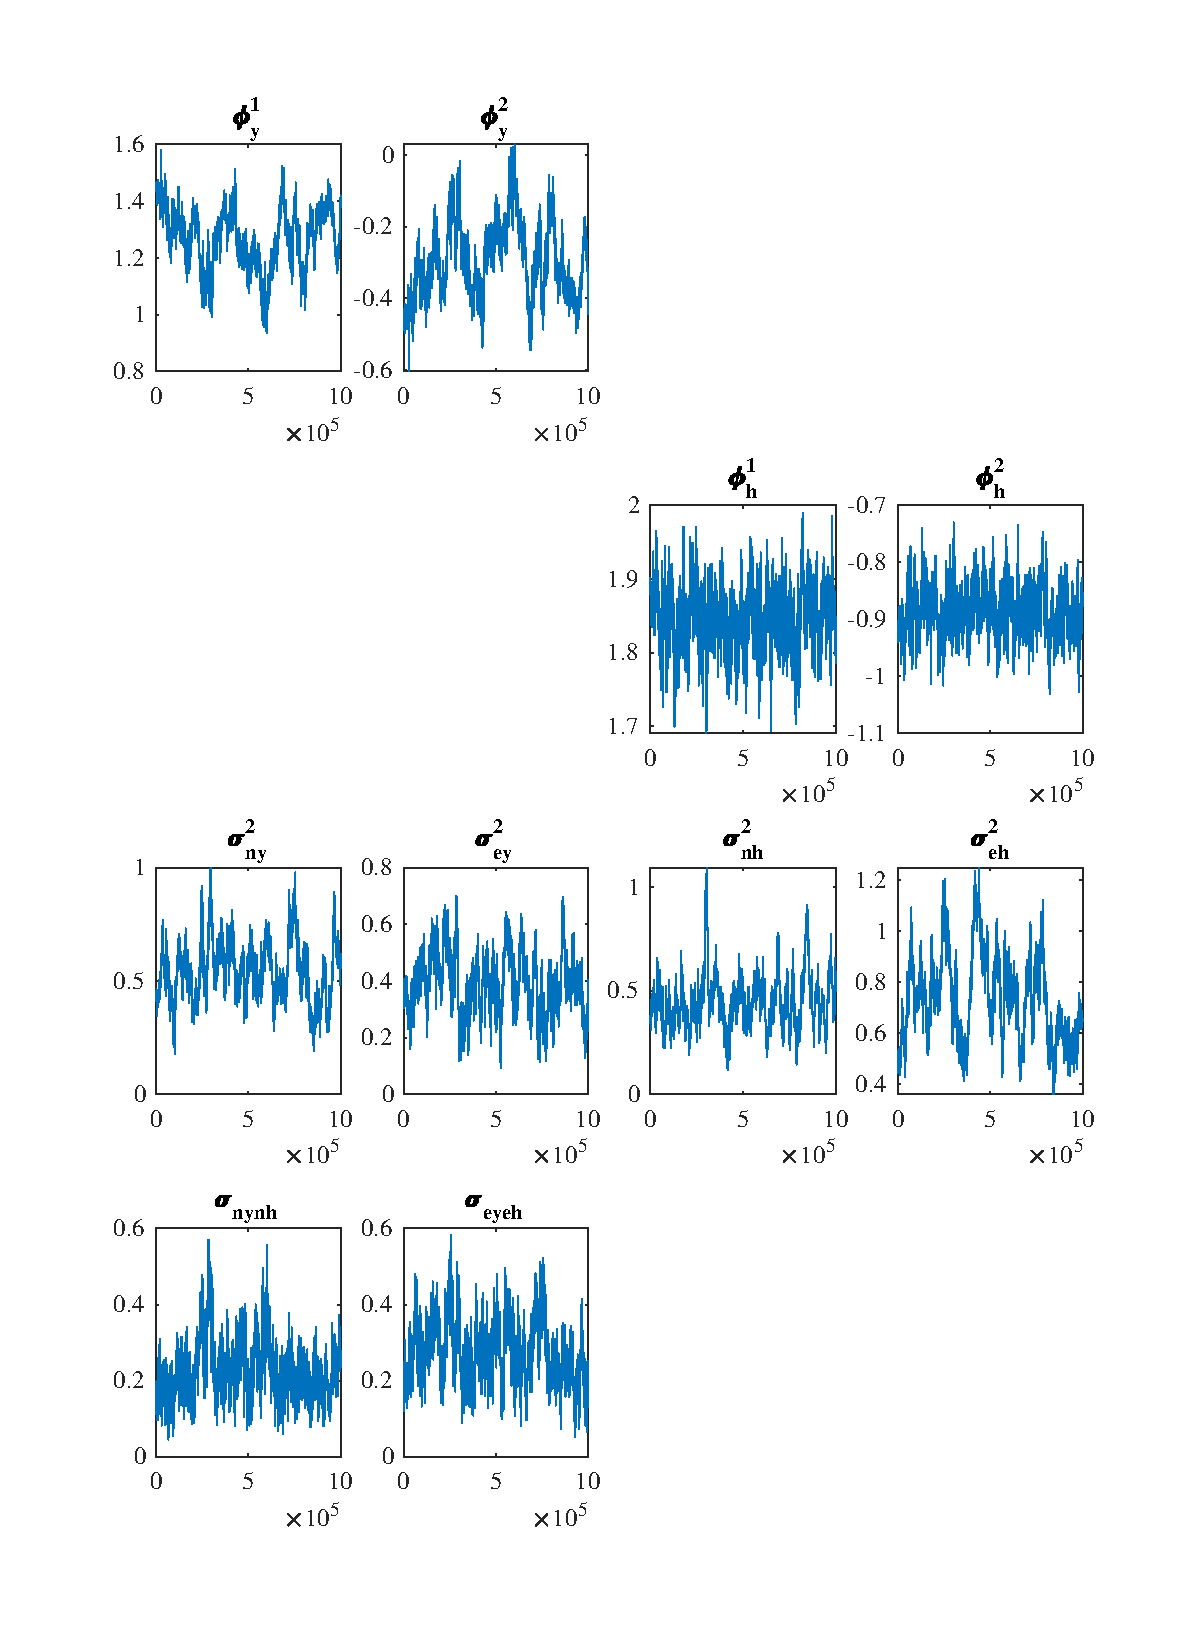
\includegraphics[width=0.85\linewidth]{../../Regression/Bayesian_UC_VAR2_nodrift/OutputData/posteriorchain_US} 

}

\caption{US VAR(2)}\label{fig:unnamed-chunk-18}
\end{figure}

\begin{figure}

{\centering 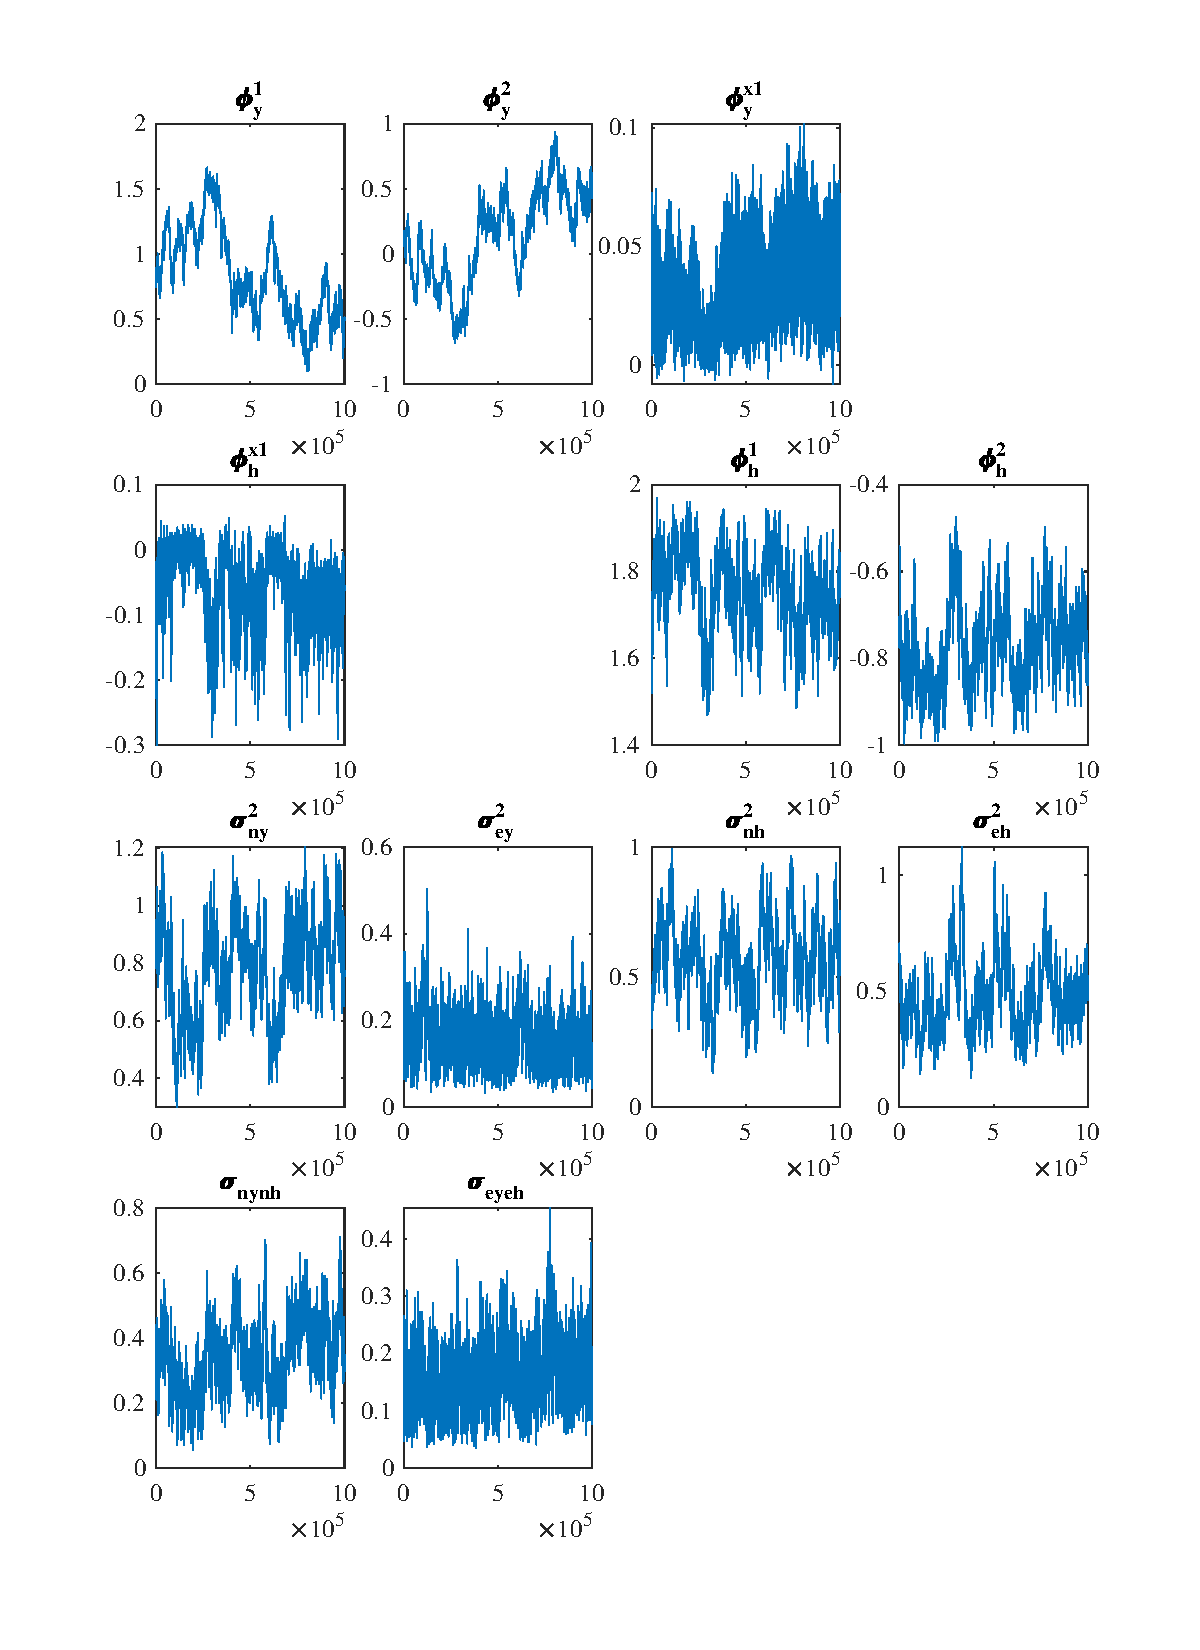
\includegraphics[width=0.85\linewidth]{../../Regression/Bayesian_UC_VAR2_nodrift_Crosscycle1lag/OutputData/posteriorchain_US} 

}

\caption{US VAR(2) 1 cross-lag}\label{fig:unnamed-chunk-19}
\end{figure}

\begin{figure}

{\centering 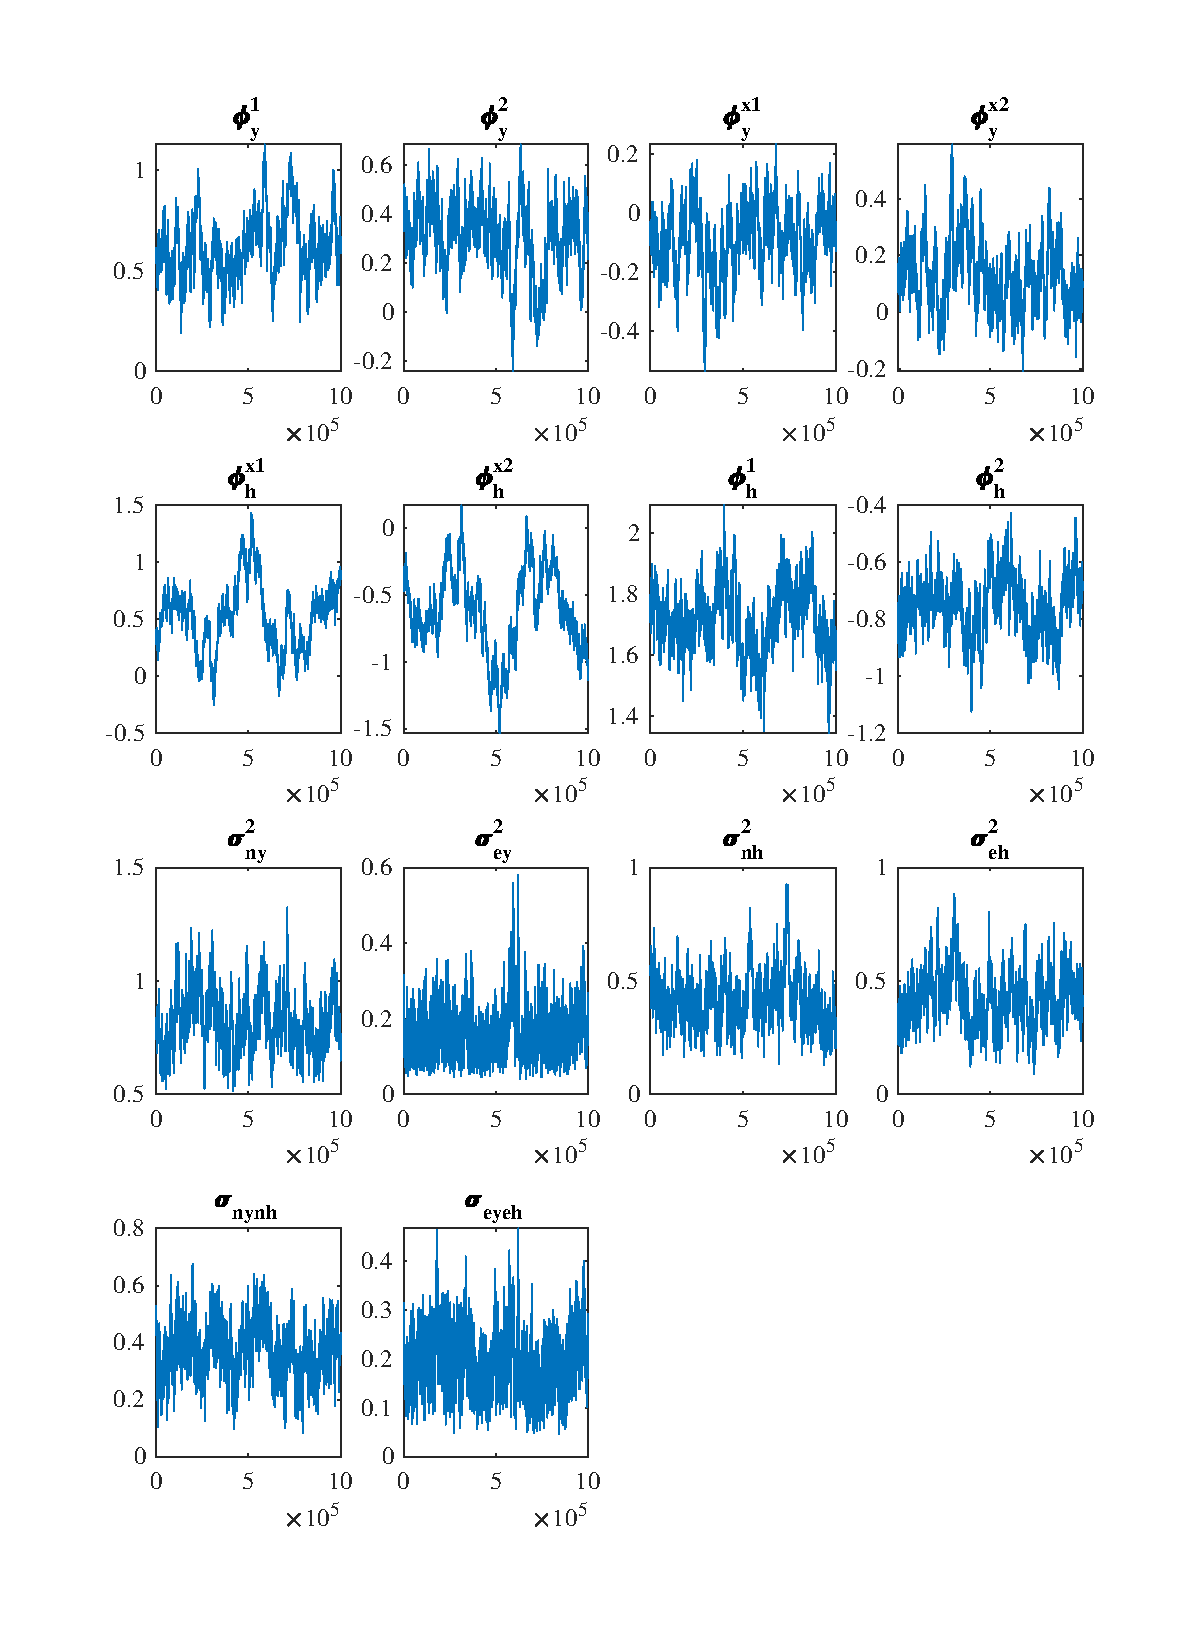
\includegraphics[width=0.85\linewidth]{../../Regression/Bayesian_UC_VAR2_nodrift_Crosscycle2lags/OutputData/posteriorchain_US} 

}

\caption{US VAR(2) 2 cross-lags}\label{fig:unnamed-chunk-20}
\end{figure}

\end{document}
